%%% File encoding is UTF8

%%% If you use this template then please give credit like this:
%%% ----------------------------
% LaTeX code inspired by the LaTeX Thesis Template by Manuel Kuehner 
% www.bedienhaptik.de/latex-template/
%%% ----------------------------

% ##############################################
% Start: Template Preamble
% ##############################################
%

% Documentclass definition
%%% File encoding is UTF8
%%% You can use special characters just like ä,ü and ñ

% KOMA-Script class 'scrbook'
% Link to the documentation: 
% German: http://mirrors.ctan.org/macros/latex/contrib/koma-script/doc/scrguide.pdf
% English: http://mirrors.ctan.org/macros/latex/contrib/koma-script/doc/scrguien.pdf
% CTAN: http://www.ctan.org/pkg/koma-script
% Author of the KOMA-Script family is Markus Kohm
\documentclass[paper=letter % Letter is "carta"
			 , fontsize=10pt % Arial 10 for all text.
			 , headings=big
			 , parskip=half-
			%, noparskip % No par skip. If yes park skip the command is parskip
			%, numbers=noendperiod % 2.3.1 vs 2.3.1. (no dot after the last chapter number)
			 , numbers=endperiod
	         , twoside=false
			% , toc=bibliography % Bibliography appears in Table of Contents (without a number)
			% , toc=listof % List of Figures and List of Tables appear in Table of Contents
			% , chapterprefix=true
			 , chapterprefix=false
			% , bibliography=totoc % The bibliography will have an entry at the table of contents but no number.
			 , numbers=noenddot
			 , titlepage=simple
			 , headings=onelinechapter
			 , version=last % Use latest version of the KOMA-Script
			 , final
]{scrbook}

\RedeclareSectionCommand[
afterskip=\parskip]{chapter}
\RedeclareSectionCommand[
beforeskip=\parskip
, afterskip=0.1\parskip]{section}
\RedeclareSectionCommand[
beforeskip=1.1\parskip plus 3mm
, afterskip=0.1\parskip]{subsection}


\KOMAoption{bibliography}{leveldown}

\newcommand{\mychapter}[1]{%
	\chapter{#1}
	\addcontentsline{lof}{chapter}{%
		Figuras del Capítulo \thechapter: #1 \vspace{10pt}
	}
}

\addtokomafont{section}{\large}
\addtokomafont{subsection}{\normalsize}  %1.1.1 Minus size: 10 % normalsize is 10

%REVISAR
\usepackage[compact]{titlesec}

% Titles in the chapters, not in TOC.
\titleformat{\chapter}
{\bfseries\Large\vspace*{-4.0cm}}	% Formato título
{	% Contenido de la etiqueta
	\filright
	\Large\MakeUppercase\chaptertitlename\ \thechapter.\ 
}
{0pt} % Espacio mínimo entre etiqueta y cuerpo
{\filright\MakeUppercase} % Código que precede al cuerpo del título
[\vspace{1.5pt}] % Margen de 1.5pt

\titleformat{\section}
{\bfseries\large\vspace{2pt}}
{\large\MakeUppercase\thesection\ \vspace{2pt} } % 3 espacios luego del titulo de una seccion
{0pt}
{\MakeUppercase}
[\vspace*{0.5cm}]

\titleformat{\subsection}
{\bfseries\normalsize\vspace{2pt}} % 3 espacios luego del titulo de una seccion
{\normalsize\thesubsection\ }
{0pt}
{\vspace*{0.5cm}}

\titleformat{\subsubsection}
{\itshape\normalsize\vspace{1.0cm}}
{\itshape\thesubsubsection\ }
{0pt}
{\vspace*{0.5cm}\itshape}

\titlespacing*{\chapter} {0pt}{85pt}{20pt} 
\titlespacing*{\section} {0pt}{6.5ex plus 1ex minus .2ex}{2.3ex plus .2ex}
\titlespacing*{\subsection} {0pt}{6.5ex plus 1ex minus .2ex}{2.3ex plus .2ex}
\titlespacing*{\subsubsection}{0pt}{3.25ex plus 1ex minus .2ex}{1.5ex plus .2ex}
\titlespacing*{\paragraph} {0pt}{3.25ex plus 1ex minus .2ex}{1em}
\titlespacing*{\subparagraph} {\parindent}{3.25ex plus 1ex minus .2ex}{1em}


% Loading additional packages from the KOMA-Script family
%%% File encoding is UTF8
%%% You can use special characters just like ä,ü and ñ

% Special KOMA-Script package - I added it because I also use the float package in this template, see: 
% http://tex.stackexchange.com/questions/51867/koma-warning-about-toc
% CTAN: http://www.ctan.org/tex-archive/macros/latex/contrib/koma-script/doc
\usepackage{scrhack}

% Better support for marginnotes
% new command: \marginnote
% LaTeX standard command: \marginpar
% CTAN: http://www.ctan.org/pkg/marginnote
\usepackage{marginnote}

% Extended header and footer support
% CTAN: http://www.ctan.org/pkg/scrpage2
\usepackage[automark
  		  , ilines
		  , headsepline
		  , footsepline
]{scrpage2}

\usepackage{setspace}
\onehalfspace

% Page layout definition
%%% File encoding is UTF8
%%% You can use special characters just like ä,ü and ñ

% User friendly interface to change layout parameters
% CTAN: http://www.ctan.org/pkg/geometry
\usepackage{geometry}
\geometry{%
	%bottom=30mm,
	, showframe=false % For debugging: try true and see the layout frames
	%, margin=30mm
	%, marginparsep=3mm
	%, marginparwidth=20mm
	, headheight=14pt
	, top=2.5cm
	, bottom=2.5cm 
	, left=4cm
	, right=2.5cm
	, letterpaper
}



% Standard packages
%%% File encoding is UTF8
%%% You can use special characters just like ä,ü and ñ

% Input encoding is 'latin1' (Latin 1 - also known as ISO-8859-1)
% CTAN: http://www.ctan.org/pkg/inputenc
% 
% A newer package is available - you may look into:
% \usepackage[x-iso-8859-1]{inputenc}
% CTAN: http://www.ctan.org/pkg/inputenx
%\usepackage[latin1]{inputenc}
\usepackage[utf8]{inputenc}

% Font Encoding is 'T1' -- important for special characters such as Umlaute ü or ä and special characters like ñ (enje)
% CTAN: http://www.ctan.org/pkg/fontenc
\usepackage[T1]{fontenc}

% Language support for 'english' (alternative 'ngerman' or 'french' for example)
% This case is in spanish
% CTAN: http://www.ctan.org/pkg/babel
%\usepackage[english]{babel} 
\usepackage[spanish
          , es-tabla
          , es-noindentfirst]{babel} 

% Doing calculations with LaTeX units -- needed for the vertical line in the footer
% CTAN: http://www.ctan.org/pkg/calc
\usepackage{calc}

% Extended graphics support 
% There is also a package named 'graphics' - watch out!
% CTAN: http://www.ctan.org/pkg/graphicx
\usepackage{graphicx}

% Extendes support for floating objects (tables, figures), adds the [H] placing option (\begin{figure}[H]) which palces it "Here" (without any doubt).
% CTAN: http://www.ctan.org/pkg/float
\usepackage{float}

% Extended color support
% I use the command \definecolor for example. 
% Option 'Table': Load the colortbl package, in order to use the tools for coloring rows, columns, and cells within tables.
% CTAN: http://www.ctan.org/pkg/xcolor
\usepackage[table]{xcolor} 

% Nice tables
% CTAN: http://www.ctan.org/pkg/booktabs
\usepackage{booktabs}

\usepackage{colortbl}

\usepackage{multirow,siunitx}

% Better support for ragged left and right. Provides the commands \RaggedRight and \RaggedLeft. 
% Standard LaTeX commands are \raggedright and \raggedleft
% http://www.ctan.org/pkg/ragged2e
\usepackage{ragged2e}

% Create function plots directly in LaTeX
% CTAN: http://www.ctan.org/pkg/pgfplots
\usepackage{pgfplots}
\pgfplotsset{compat=1.11}

% Main Font used: Arial
\usepackage{uarial}
\usepackage[expert]{mathdesign}
\renewcommand{\familydefault}{\sfdefault}

% tocloft ? Control table of contents, figures, etc
% CTAN: https://ctan.org/pkg/tocloft
%\usepackage{tocloft}

% Configure Microtype
\usepackage[activate={true,nocompatibility},final,tracking=true,kerning=true,spacing=true,factor=1100,stretch=10,shrink=10]{microtype}
% activate={true,nocompatibility} - activate protrusion and expansion
% final - enable microtype; use "draft" to disable
% tracking=true, kerning=true, spacing=true - activate these techniques
% factor=1100 - add 10% to the protrusion amount (default is 1000)
% stretch=10, shrink=10 - reduce stretchability/shrinkability (default is 20/20)

\SetExtraKerning[unit=space]
{encoding={*}, family={bch}, series={*}, size={footnotesize,small,normalsize}}
{\textendash={400,400}, % en-dash, add more space around it
	"28={ ,150}, % left bracket, add space from right
	"29={150, }, % right bracket, add space from left
	\textquotedblleft={ ,150}, % left quotation mark, space from right
	\textquotedblright={150, }} % right quotation mark, space from left

\SetExtraKerning[unit=space]
{encoding={*}, family={qhv}, series={b}, size={large,Large}}
{1={-200,-200}, 
	\textendash={400,400}}

% Use French spacing
\frenchspacing



% https://www.ctan.org/pkg/biblatex-ieee
\usepackage[backend=biber
		  %, style=ieee % Esta bien, pero no agrupa las citaciones
		  %, style=numeric-comp %Revisar, porque algunas referencias no las tira correctas
		  %Antes: IEEE
		  %, bibstyle=ieee  %Combinacion de ambas
		  %, citestyle=numeric-comp
		  %AHORA: APA
		  , style=apa
		  , hyperref=true
		  , url=false
		  , isbn=false
		  , backref=true
		 %, style=custom-numeric-comp
		  , citereset=chapter
		  , maxcitenames=3
		  , maxbibnames=100
		  , block=none
		  %, sorting=none % El orden de las citas en IEEE es según el orden de aparicion en el texto
		  , sortcites=true
		  , sorting=nyt
		  % APA no tiene referencias cruzadas, si se quiere desactivar, comentar apabackref
		  , apabackref=true
		  , language=spanish
]{biblatex}
\bibliography{bibfile}

% Separacion entre entradas de la referencia
\setlength\bibitemsep{\baselineskip}

\DeclareLanguageMapping{spanish}{spanish-apa}

\usepackage[style=english]{csquotes}

%TODO: Cambiar de bibliografia a Referencias Bibliograficas
\renewcommand\bibname{Referencias Bibliogr\'aficas}
\DefineBibliographyStrings{spanish}{%
	andothers = {\em et\addabbrvspace al\adddot}
}

\AtEveryBibitem{%
	\ifboolexpr{test {\ifentrytype{article}} and not test {\iffieldundef{doi}}}
	{\clearfield{number}}
	{}%
}

\usepackage{pgfplotstable}

%FIX: dont work
\usepackage[noabbrev,capitalize,nameinlink,spanish]{cleveref}
\crefname{table}{\spanishtablename}{\spanishtablename}

\usepackage{subcaption}

\usepackage{neuralnetwork}

\usepackage[linesnumbered
		   , algoruled
	       , vlined
	       , boxed
	       , algochapter
	       , commentsnumbered
	       , spanish
	       , onelanguage
]{algorithm2e}

\usepackage{pgfgantt}
\ganttset{
	, y unit title=0.5cm
	, y unit chart=0.7cm
	, vgrid,hgrid
	, progress=today
	, group/.append style={orange}
	, milestone/.append style={red}
	, progress label node anchor/.append style={text=red}
	, bar/.style={draw=black, fill=gray!50}
	, incomplete/.style={draw=black, fill=white}
	, title height=1
	, title label font=\bfseries\footnotesize
	, bar/.style={fill=black}
	, bar height=0.7
	, today label=HOY
	, group right shift=0
	, group top shift=0.7
	, group height=.3
	, group peaks width={0.2}
	, inline
} 

\usepackage{graphicx}
\usepackage{xcolor}

\usepackage{amsmath,amssymb}


% Use Spanish file for hyphenation
\hyphenation{hyph-es}

% ####-Important-####
%
% Definition of the two main colors
% -----------------------
% The corresponding xcolor package ist loaded in the file 
% 01_Preamble/StandardPackages.tex
%
% ####-Important-####
%\definecolor[named]{myColorMainA}{RGB}{0,26,153}
%\definecolor[named]{myColorMainB}{RGB}{174,49,54}
\definecolor[named]{myColorMainA}{RGB}{0,0,0}
\definecolor[named]{myColorMainB}{RGB}{0,0,0}
\definecolor{mylinkcolor}{RGB}{5,123,10}
\definecolor{mycitecolor}{RGB}{5,10,123}

% colors
\definecolor{gray75}{gray}{0.75}
\definecolor{gray90}{gray}{0.90}
\definecolor{darkblue}{rgb}{0,0,0.5}
\definecolor{darkgreen}{rgb}{0,0.5,0}
\definecolor{green}{rgb}{0.2,0.8,0.2}
\definecolor{red}{rgb}{1.0,0.3,0.0}
\definecolor{orange}{rgb}{1.0,0.6,0.0}

% Customization of 
% - Floating Objects (Caption) 
% - Table of Contents (TOC)
% - List of Figures
% - List of Tables
% - Headings (like chapter, section, etc.)
% - Bibliography Style
%%% File encoding is UTF8
%%% You can use special characters just like ä,ü and ñ

% ##############################################
% Start: Table of Contents (TOC) Customization
% ##############################################
%

% Level for numbered captions
\setcounter{secnumdepth}{5}

% Level of chapters that appear in Table of Contents
\setcounter{tocdepth}{5} % bis wohin ins Inhaltsverzeichnis aufnehmen
% -2 no caption at all
% -1 part
% 0  chapter
% 1  section    
% 2  subsection 
% 3  subsubsection
% 4  paragraph
% 5  subparagraph

% KOMA-Script code to adjust TOC
% Applying the color 'myColorMainA' which is defined in the main file (MainFile.tex)
\makeatletter
%Dont use color
\addtokomafont{chapterentrypagenumber}{\color{myColorMainA}}
\addtokomafont{chapterentry}{\color{myColorMainA}}
\makeatother

\renewcaptionname{spanish}{\contentsname}{\hfill\bfseries\Large Tabla de Contenidos \hfill} % Table of contents in spanish
\renewcaptionname{spanish}{\listfigurename}{\hfill\bfseries\Large \'Indice de Figuras \hfill}    %Figures
\renewcaptionname{spanish}{\listtablename}{\hfill\bfseries\Large \'Indice de Tablas \hfill}        %Tables

%Funciona
\makeatletter
\let\oldaddchaptertocentry\addchaptertocentry
\renewcommand{\addchaptertocentry}[2]{%
	\oldaddchaptertocentry{}{\@chapapp{} #1. #2}}
\let\oldaddparttocentry\addparttocentry
\renewcommand{\addparttocentry}[2]{%
	\oldaddchaptertocentry{}{\partname{} #1. #2}}

\RedeclareSectionCommand[tocindent=5.5em]{section}
\RedeclareSectionCommand[tocindent=7.8em]{subsection}

\makeatother

\makeatletter
\newcommand{\chapterwithfigures}{\addxcontentsline{lof}{chapteratlist}[{\thechapter}]{\scr@ds@tocentry}}%
\makeatother

%
% #######################
% End: Table of Contents (TOC) Customization
% #######################

% ##############################################
% Start: Floating Object Customization
% ##############################################
%

% Extended support for catioons of figures and tables etc.
% CTAN: http://www.ctan.org/pkg/caption
\usepackage[font={small}
		  %, labelfont={bf,sf}
		  , labelfont={sf}
		  , format=hang % try plain or hang
		  , margin=5pt
]{caption}
%

\newcommand{\englishword}[1]{\textit{#1}}

\newcommand{\ingles}[1]{\textit{#1}}
\newcommand{\producto}[1]{\textit{#1}}
\newcommand{\tecnologia}[1]{\textit{#1}}

\newcommand*{\captionsource}[2]{%
	\caption[{#1}]{#1}
	\par\centering\small{Fuente: #2.}
}

\newcommand*{\captiontable}[2]{%
	\captionabove[{#1}]{#1 \par\centering \small{Fuente: #2.}}
}

% Make Uppecase section title
\addtokomafont{section}{\MakeUppercase}

% Tables with PGFPlots
\usepackage{pgfplotstable} % Generates table from .csv
\usepgfplotslibrary{colorbrewer}
\usepgfplotslibrary{statistics}

\pgfplotsset{cycle list/Dark2}
\pgfplotsset{cycle list/Dark2-5}

% Table: htb: place here, top, or bottom, BUT NEVER at other page
%Args: 
% 1: Caption
% 2: Source
% 3: CSV File (separated by semicolons ;)
% 4: Label command
\newcommand{\insertTableFile}[4]{
	\begin{table}[htb]
	\centering
	\captiontable{#1}{#2}
	\pgfplotstabletypeset[
	every even row/.style={
		before row={\rowcolor[gray]{0.9}}},
	every head row/.style={
		before row=\toprule,after row=\midrule},
	every last row/.style={
		after row=\bottomrule},
	col sep=semicolon, 
	string type]{#3}
	#4 % Label command		
	\end{table}
}


% Arg 1: X label
% Arg 2: Y label
% Arg 3: Filename
% Arg 4: Caption
% Arg 5: Source
% Arg 6: Label

\newcommand{\plotFile}[3]{
	\pgfplotsset{cycle list/Dark2}
	\begin{figure}[htb]
	\centering
	\begin{tikzpicture}
	\begin{axis}[
	xlabel={#1},
	ylabel={#2},
	xmin=0,
	ymin=0,
	ymax=1,
	legend style = {
		legend pos = outer north east,
	},
	%cycle list name=Dark2,
	width=0.7\textwidth
	]
	\legend{Legend 1}
	\pgfplotstableread{#3}\leg1;
	\addplot+ [
	cycle list name=Dark2,
	mark=square*
	] table []{\leg1};
	\end{axis}
	\end{tikzpicture}
	%\captionsource{#4}{#5}
	%#6	
	\end{figure}

}

\newcommand{\correcion}[1]{\hl{#1}}
\newcommand{\currentYear}{2017}
\newcommand{\fuentePropia}{Elaboración propia, (\currentYear)}


%% References
\newcommand{\tab}[1]{Tabla~\ref{#1}}
\newcommand{\tabla}[1]{Tabla~\ref{#1}}
\newcommand{\fig}[1]{Figura~\ref{#1}}
\newcommand{\alg}[1]{Algoritmo~\ref{#1}}
\newcommand{\eq}[1]{Ecuación~\ref{#1}}


% #######################
% End: Floating Object Customization
% #######################

% ##############################################
% Start: Headings Customization
% ##############################################
%

% KOMA-Script code to customize the headings
% Applying the color 'myColorMainA' which is defined in the main file (MainFile.tex)
%\addtokomafont{chapter}{\color{myColorMainA}}
%\addtokomafont{section}{\color{myColorMainA}}
%\addtokomafont{subsection}{\color{myColorMainA}}
%\addtokomafont{subsubsection}{\color{myColorMainA}}
%\addtokomafont{paragraph}{\color{myColorMainA}}
%\addtokomafont{subparagraph}{\color{myColorMainA}}

% #######################
% End: Headings Customization
% #######################


% Customization of the header, footer and teh margin note
%%% File encoding is UTF8
%%% You can use special characters just like ä,ü and ñ

% Custom command fpr the margin notes: \myMarginnote{Your Text}
% Comment on the \lineskiplimit=-\maxdimen:
% See http://tex.stackexchange.com/questions/49072/
% Without it the line spacing of the normal text was changed (ugly).
\newcommand{\myMarginnote}[1]{%
	\marginnote{% needs marginnote package
		\ifthispageodd{\RaggedRight}{\RaggedLeft}% needs ragged2e package
		\color{myColorMainB}%
		\lineskiplimit=-\maxdimen% 
		\normalfont\sffamily\scriptsize%
		#1}%
}

% ##############################################
% Start: Header and Footer Customization
% ##############################################
%



% KOMA-Script code for header and footer font
\setkomafont{pageheadfoot}{%
	\normalfont\sffamily\bfseries
	}
\setkomafont{pagefoot}{%
	\normalfont\sffamily
	}
\setkomafont{pagenumber}{%
	\normalfont\rmfamily
	}

% Define width of header
%\setheadwidth[0pt]{textwithmarginpar}

% Define with of header line
\setheadsepline{0.4pt}

% Define width of footer
\setfootwidth[0pt]{text}
% Define with of footer line (here: no line)
\setfootsepline[text]{0pt}

% Some calculations
% calc package is needed which is loaded here: 01_Preamble/CommonPackages.tex
% If you want to understand the calculations visit:
% http://en.wikibooks.org/wiki/LaTeX/Page_Layout
\newlength{\myLenghthFootAbstand}
\setlength{\myLenghthFootAbstand}{\paperheight-1in-\topmargin- \headheight-\headsep-\textheight-\footskip}
\newlength{\myLenghthTemp}
\setlength{\myLenghthTemp}{\myLenghthFootAbstand+\baselineskip}

% Define content of header and footer
% Using some scrpage2 commands here. The scrpage2 package is loaded here: 01_Preamble/KOMA-Script-Packages.tex
% Some LaTeX magic...
% Clear all defaults
\clearscrheadfoot
% Header
\ohead{\textcolor{myColorMainA}{\headmark}}

% Footers
\lefoot[\pagemark]{\pagemark}
\rofoot[\pagemark]{\pagemark}

\automark[section]{chapter}


%
% #######################
% End: Header and Footer Customization
% #######################

% Optimize paragraphs (avoid overfull... warnings)
%%% File encoding is UTF8
%%% You can use special characters just like ä,ü and ñ

% This is an suggestion from Axel Reichert (LaTeX package author)
% See CTAN: http://www.ctan.org/author/reichert
% See CTAN: http://www.ctan.org/pkg/l2tabu-english (Cgapter: 1.8 Should I use \sloppy?)

\tolerance 1414
\hbadness 1414
\emergencystretch 1.5em
\hfuzz 0.3pt
\widowpenalty=10000
\vfuzz \hfuzz
\raggedbottom

% Interlineado de 1.5:
\renewcommand{\baselinestretch}{1.5}

\setlength{\parindent}{1em}
%\setlength{\parindent}{4em}
\setlength{\parskip}{\baselineskip}
%\parskip = \baselineskip
%\setlength{\parskip}{0.3em}
%\parskip = 2\baselineskip % no shrink and no stretch

% PDF related packages
%%% File encoding is UTF8
%%% You can use special characters just like ä,ü and ñ

% Package for PDF features such as bookmarks and hyperlinks. 
% Important: Should be loaded at the end.
% CTAN: http://www.ctan.org/pkg/hyperref
\usepackage[bookmarks			   % Create bookmarks
		  , bookmarksopen=true,    % Unfold bookmatk tree in PDF viewer when document is opened
		  , bookmarksopenlevel=1   % Level of unfolding
		  , bookmarksnumbered=true % Number bookmarks
		  , hidelinks              % do not highlight hyperlinks -- looks ugly
		  , pdfpagelabels=true     % See manual...
		  , plainpages=false       % See manual...
		  , hyperfootnotes=true    % Hyperlinks for footnotes
		  , hyperindex=true        % Indexeinträage verweisen auf Text
		 % Links, solo en version PDF virtual
		  , colorlinks=true
		  , linkcolor=darkblue     % Color of internal links
		  , citecolor=darkblue     % Color of links to bibliography
		  , filecolor=darkblue     % Color of file links
		  , urlcolor=darkgreen     % Color of external links
		  , pdftex
		  , pdftitle={Modelo predictivo del desempeño de búsqueda de información en línea en estudiantes de educación básica}
		  , pdfauthor={Gonzalo Javier Martinez Ramirez}
		  , pdfsubject={Tesis de grado}
		  , pdfkeywords={Alfabetización informacional, competencias de investigación en línea, comportamiento de estudiantes, minería de datos, modelos de clasificación.}
		  , pdfcreator={pdflatex}
]{hyperref}

% PDF related packages
%%% File encoding is UTF8
%%% You can use special characters just like ä,ü and ñ

% Package to create test text -- just for demonstration purposes
% The command \blindtext produces a test text -- good for testing the layout
% CTAN: http://www.ctan.org/pkg/blindtext
\usepackage[]{blindtext}
% The custom command \myMarginnote is defined in the file: 
% 01_Preamble/HeaderFooterMarginnote.tex
\renewcommand{\blindmarkup}[1]{\myMarginnote{#1}}

% Bibliography
%%% File encoding is UTF8
%%% You can use special characters just like ä,ü and ñ

%% Bibliography style

% Prints author names as small caps
%\renewcommand{\mkbibnamefirst}[1]{\textsc{#1}}
%\renewcommand{\mkbibnamelast}[1]{\textsc{#1}}
%\renewcommand{\mkbibnameprefix}[1]{\textsc{#1}}
%\renewcommand{\mkbibnameaffix}[1]{\textsc{#1}}

% document preamble
% removes period at the very end of bibliographic record
%\renewcommand{\finentrypunct}{}

%\renewcommand{\newunitpunct}{\addspace\midsentence}

\DeclareUnicodeCharacter{00A0}{ }

\DefineBibliographyStrings{english}{%
	backrefpage  = {\lowercase{s}ee p.}, % for single page number
	backrefpages = {\lowercase{s}ee pp.} % for multiple page numbers
}

\DefineBibliographyStrings{spanish}{%
	backrefpage  = {\lowercase{v}er pág.}, % for single page number
	backrefpages = {\lowercase{v}er págs.} % for multiple page numbers
}


%\DeclareFieldFormat{journaltitle}{\mkbibemph{#1},} % italic journal title with comma
%\DeclareFieldFormat[inbook,thesis]{title}{\mkbibemph{#1}\addperiod} % italic title with period
%\DeclareFieldFormat[article]{title}{#1} % title of journal article is printed as normal text

% makes volume of journal bold and adds colon
%\DeclareFieldFormat[article]{volume}{\textbf{#1}\addcolon\space}

% removes pagination (p./pp.) before page numbers
%\DeclareFieldFormat{pages}{#1}

%%
% Footnote
%

% new command \sjcitep prints footnote citation above punctuation
\newlength{\spc} % declare a variable to save spacing value
\newcommand{\sjcitep}[2][]{% new command with two arguments: optional (#1) and mandatory (#2)
	\settowidth{\spc}{#1}% set value of \spc variable to the width of #1 argument
	\addtolength{\spc}{-1.8\spc}% subtract from \spc about two (1.8) of its values making its magnitude negative
	#1% print the optional argument
	\hspace*{\spc}% print an additional negative spacing stored in \spc after #1
	\supershortnotecite{#2}}% print (cite) the mandatory argument

%
% #######################
% Ende: Template Preamble
% #######################

% ##############################################
% Start: Document
% ##############################################
%
% ------------------------------------------------------------------
\begin{document}

% Title page
%%% File encoding is ISO-8859-1 (also known as Latin-1)
%%% You can use special characters just like ä,ü and ñ

% Title page using \maketitle (a more flexible alternative is the titlepage environment)
%\title{PHD Thesis}
%\subtitle{\LaTeX{} template by Manuel Kuehner\\ \url{www.bedienhaptik.de/latex-template/}}
%\author{Manuel Kuehner}
%\date{01.01.2015}


%\maketitle
\def\alumno#1{Gonzalo Martinez Ramirez}
\def\rut#1{18.045.598\ -\ 1}
\def\ingreso#1{2010}
\def\fono#1{(+56)\ 9\ -\ 96112973}
\def\mail#1{gonzalo.martinez@usach.cl}
\def\profesorguia#1{Roberto Ignacio González Ibáñez}

\newgeometry{top=4cm, bottom=2.5cm, left=4cm, right=2.5cm}
\begin{titlepage}
	\begin{center}
		{\Large\bfseries UNIVERSIDAD DE SANTIAGO DE CHILE} \\ 
		{\large\bfseries FACULTAD DE INGENIERÍA} \\
		{\large\bfseries Departamento de Ingeniería Informática} \\

		\begin{picture}(18,4)(0,40)
		\put(160,50){
\includegraphics[width=0.15\textwidth]{03_GraphicFiles/logo-onlyescudo-usach-bw}}
		\end{picture}
		
		% ----------------------------------------------------------------
		%\vspace{5cm}
		\vspace*{\fill}
		{\Large\bfseries \MakeUppercase MODELO PREDICTIVO DEL DESEMPEÑO DE BÚSQUEDA DE INFORMACIÓN EN LÍNEA EN ESTUDIANTES DE EDUCACIÓN BÁSICA} \\ %[5pt]
		\vfill
		{\bfseries Gonzalo Javier Martinez Ramirez}
		\vspace*{\fill}
		% ----------------------------------------------------------------
	
		\vfill
		\begin{flushright}
			\begin{tabular}[t]{rl}
				%Nombre: & Gonzalo Javier Martinez Ramirez \\
				%R.U.T.: & 18.045.598-1 \\
				%A\~no Ingreso: & 2010 \\
				%Tel\'efono: & (+56) 9 96112973 \\
				%E-mail: & gonzalo.martinez@usach.cl \\
				Profesor guía: & \profesorguia \\ 
			\end{tabular}
		\end{flushright}
	
		\vspace{1cm}
		\hspace{6.12cm}
		\begin{tabular}{p{7.2cm}}
		Tesis de grado presentado en conformidad a los requisitos para obtener el grado de Magíster en Ingeniería Informática.
		\end{tabular}
		%\begin{flushright}
		%	\begin{tabular}[t]{rl}
		%	Tesis de grado presentado en conformidad a los requisitos para obtener el grado de Magíster en Ingeniería Informática.
		%	\end{tabular}
		%\end{flushright}

		\vfill
		{Santiago\ \textendash \ Chile} \\
		{2017}
	\end{center}
\end{titlepage}
\restoregeometry
% Empty page after title page
\cleardoublepage

% Activate header and footer defined in the file:
% 01_Preamble/HeaderFooterMarginnote.tex
\pagestyle{scrheadings}

% Activate roman numbering (e. g. xii)	
\pagenumbering{roman}

% Start with page 1 (I)
\setcounter{page}{1}

% Abstract
%%% File encoding is UTF8
%%% You can use special characters just like ä,ü and ñ

% Chapter without numbering but with appearance in the Table of Contents
% \addchap is a command from KOMA-Script
%\addchap*{Abstract}

\chapter*{\centerline{Resumen}} \vspace{-6em}
Durante la última década, debido a los rápidos avances de las tecnologías de la información y comunicación ha aumentado la cantidad de recursos digitales en Internet, la diversidad de fuentes de información, además, se ha facilitado el acceso a estos. Asimismo, las búsquedas \ingles{web} han pasado a ser parte de las tareas comunes que realizan los estudiantes de los planteles educativos. Considerando la diversidad de fuentes de información y tipos de recursos en línea, resulta necesario desarrollar competencias informacionales durante el proceso de formación en los distintos niveles educativos (primaria, secundaria y universitaria).

En el marco del proyecto iFuCo (\ingles{Enhancing learning and teaching future competences of online inquiry in multiple domains}), formado por investigadores de Chile y Finlandia, el cual desea investigar y modelar los comportamientos y competencias de investigación en línea de estudiantes de enseñanza básica, se propone la construcción de un modelo de predicción del desempeño de búsqueda de información en línea en estudiantes de educación básica el cual se vaya perfeccionando a través del registro de datos históricos y que de una retroalimentación de forma continua.


%La investigación será guiada por la metodología KDD con el fin de descubrir patrones en los datos que permitan la creación de un modelo de predicción del comportamiento de búsqueda. Además, para apoyar el proceso de investigación, se desarrollará una plataforma que funcione como extensión de la plataforma NEURONE (\ingles{oNlinE inqUiry expeRimentatiON systEm}). La plataforma propuesta alimentará y perfeccionará el modelo de predicción y entregará predicciones en tiempo real. Esta plataforma se guiará bajo la metodología RAD (\ingles{Rapid Application Development}) la cual se orienta a un desarrollo iterativo e incremental para la rápida construcción de prototipos de \ingles{software}.

\par\noindent
{\bfseries Palabras Claves\/}: Alfabetización informacional, competencias de investigación en línea, comportamiento de estudiantes, minería de datos, modelos de clasificación.

\newpage
\chapter*{\centerline{Abstract}} \vspace{-6em}
During the last decade, due to rapid advances in information and communication technologies, the number of digital resources on the Internet has increased, and the diversity of information sources has also facilitated access to information. In addition, web searches have become part of the common tasks performed by students in schools. Considering the diversity of sources of information and types of online resources, it is necessary to develop informational competences during the training process at different levels of education (primary, secondary and university/college).

In the framework of the iFuCo project, which consists of researchers from Chile and Finland, who wishes to investigate and model online research behaviors and competencies of basic education students, we propose the construction of a prediction model of information search performance In line in students of basic education that is perfected through the registry of historical data and that of a feedback of continuous form.



\par\noindent
{\bfseries Keywords\/}: Data mining, machine learning, classification models.

% Table of Contents and Lost of Figures/Tables
%%% File encoding is ISO-8859-1 (also known as Latin-1)
%%% You can use special characters just like ä,ü and ñ

% Table of Contents (TOC)
% Special code so that it appears as a bookmark in the PDF viewer
\phantomsection
\pdfbookmark[0]{Tabla de contenidos}{toc} % <-- Please edit the name if you want a different text as a bookbarl for the Table of Contents

\microtypesetup{protrusion=false} % disables protrusion locally in the document
\tableofcontents
\listoftables 
\listoffigures
\microtypesetup{protrusion=true} % enables protrusion

\chapter{Objetivos y alcances de la solución}
\label{chp:objetivos}
% Activate arabic numbering (e. g. 12)	
\pagenumbering{arabic}
% Start with page 1 (I)
\setcounter{page}{1}

\section{Objetivo general}
\label{sec:objetivo-general}
Diseñar y evaluar un modelo predictivo del desempeño de búsqueda de información en línea de estudiantes de enseñanza básica.

\section{Objetivos específicos}
\label{sec:objetivo-especificos}

\begin{enumerate}
	\item Realizar una revisión bibliográfica sobre trabajos recientes relacionados con minería de datos en el contexto educacional.
	\item Realizar una exploración, limpieza, pre-procesamiento y transformación de los datos recopilados por la plataforma NEURONE (acrónimo de oNlinE inqUiry expeRimentatiON systEm).
	%old
	%\item Definir las características de comportamiento de búsqueda de los estudiantes para la construcción de modelos predicción.
	%new: Seleccionar características de comportamiento de búsqueda de los estudiantes para la construcción de modelos predictivos.
	\item Seleccionar características de comportamiento de búsqueda de los estudiantes para la construcción de modelos predictivos.
	%old
	%\item Comparar, seleccionar e implementar algoritmos de minería de datos, para la construcción de modelos de predicción.
	%new Construir modelos para la predicción
	\item Construir modelos para la predicción del desempeño de búsqueda en línea de estudiantes de educación básica.
	%old
	%\item Implementar los modelos de predicción del comportamiento de búsqueda en línea de estudiantes de básica.
	%new Evaluar modelos
	\item Evaluar los modelos predictivos del desempeño de búsqueda en linea de estudiantes de educación básica.
	%old
	%\item Implementar y evaluar una plataforma de enseñanza de competencias informacionales, la cual en base a los datos provistos por NEURONE prediga el desempeño de búsqueda de un estudiante.
	% new: 6. Implementar modelos en NEURONE.....
	\item Implementar los modelos predictivos en la plataforma NEURONE.
\end{enumerate}
\chapter{Descripción del problema}
\label{chp:descripcion-problema}

\section{Motivación}
\label{sec:motivacion}
%Revisar estilo OREO
Durante la última década, debido a los rápidos avances de las tecnologías de la información y comunicación (TICs, desde ahora en adelante) ha aumentado la cantidad de recursos digitales en Internet y la diversidad de fuentes de información. Además, se ha facilitado el acceso a estos. Asimismo, las búsquedas \ingles{web} han pasado a ser parte de las tareas comunes que realizan los estudiantes de los planteles educativos. En consecuencia, se ha disminuido las visitas a bibliotecas, y el uso de fuentes revisadas y editadas.

La alfabetización en información es una disciplina que se define a sí misma en base al desarrollo de destrezas, habilidades y competencias informacionales que permitan ir fortaleciendo el aprendizaje constante y el trabajo colaborativo \parencite{american2000information}. Además, favorece la capacidad de buscar, clasificar, y comprender la información, para posteriormente convertirla en conocimiento asimilado y útil. A causa de esto, el estudio, análisis y modelado de las conductas de los estudiantes en ambientes de búsqueda \ingles{web} es esencial para comprender sus niveles de alfabetización informacional \parencite{tseng2009meta}.

Actualmente, en Chile la enseñanza de competencias informacionales es cubierta en bibliotecas universitarias y cursos introductorios de mallas universitarias \parencite{marzal2015diagnostico}. De acuerdo con \cite{urra2016alfabetizacion}, los estudiantes universitarios de Chile presentan problemas con las competencias informacionales, ya que no aplican la búsqueda de información de forma crítica. Una de las posibles causas de por qué los estudiantes tienen dificultades con estas competencias es el hecho de que en los colegios y en el inicio de su educación se prioriza la reiteración de la información.

Las consecuencias de no considerar cuándo y por qué se necesita la información, dónde encontrarla, y cómo evaluarla, se ven reflejadas en la evaluación crítica de la información, y en el desempeño de los estudiantes \cite{urra2016alfabetizacion}. A causa de esto, existe la necesidad de estudiar el fenómeno de la alfabetización informacional y las competencias de investigación en línea con los objetivos de i) conocer y estudiar los comportamientos de los estudiantes en tareas de búsqueda de información en medios digitales, y ii) obtener modelos para reforzar los niveles de alfabetización informacional.

Esta propuesta de tesis se enmarca en el contexto del proyecto de investigación “\ingles{Enhancing Learning and Teaching Future Competences of Online Inquiry in Multiple Domains}” (iFuCo, desde ahora en adelante) [24], el cual pretende abordar la temática de la alfabetización informacional en estudiantes de enseñanza básica con el objetivo de estudiar sus patrones de comportamiento y ofrecer modelos curriculares adecuados respecto al tema [3].

\section{Revisión de la literatura}
\label{sec:revision-literatura}
Esta sección tiene como objetivo entregar las bases teóricas, conceptuales y empíricas que soportan el desarrollo de esta investigación. En primer lugar, se presenta el marco conceptual donde se entregan las definiciones y conceptos necesarios para abordar esta investigación. Finalmente, se presenta el estado del arte relacionado con el tema.

\subsection{Marco conceptual}

\subsection*{Alfabetización informacional}
La alfabetización informacional (conocida en ingles \ingles{information literacy}) es definida como “el grupo de habilidades en las que se requiere reconocer cuándo la información es necesaria y tener la habilidad de encontrar, evaluar y usar efectivamente dicha información necesaria” \footnote{\traduccionlibre} \parencite[p.~2]{american2000information}. Es un campo que cubre varias áreas, entre las que se destaca la alfabetización digital, las habilidades de uso de bibliotecas, la ética informacional, la lectura crítica, el pensamiento crítico, los derechos de autor, la seguridad y privacidad, entre otras. A través del estudio de estas áreas como factores que influyen a la alfabetización informacional se puede obtener una visión clara de cómo los estudiantes llevan a cabo sus tareas de obtención y selección de información.

\subsection*{Competencias de investigación en línea}
Se definen las competencias de investigación (\ingles{inquiry skills} en inglés) como “las habilidades para explorar preguntas, para poder reunir, interpretar y sintetizar diferentes tipos de información y datos, además de desarrollar y compartir una explicación para responder preguntas dadas” \footnote{\traduccionlibre} \parencite[p.~13]{national2000inquiry}. En base a este concepto nacen las competencias de investigación en línea (conocidas en inglés como \ingles{online inquiry skills}), que son una instancia específica de las competencias de investigación, pero aplicada sobre información disponible en línea \parencite{quintana2005framework}.

Las competencias de investigación en línea involucran una serie de actividades cognitivas, como generar una pregunta de investigación, buscar información relevante en colecciones digitales, evaluar y seleccionar la información encontrada, e integrar coherentemente la información seleccionada para responder la pregunta original \parencite{eisenberg1990information}.

\subsection*{Minería de datos educacional}
La minería de datos utiliza una combinación de bases de conocimientos explícita, conocimientos analíticos complejos y conocimiento de campo para descubrir las tendencias y los patrones ocultos, estas tendencias y patrones forman la base de los modelos predictivos que permiten a los analistas realizar nuevas observaciones de los datos existentes \parencite{luan2002data}. La gran cantidad de información generada hoy en día por los estudiantes permite que la minería de datos obtenga datos relevantes y, a través de métodos estadísticos y otras herramientas, relacione la información para conocer si el proceso de enseñanza aprendizaje ha dado resultados positivos. 

\textcite[p.~9]{mining2012enhancing} define la minería de datos educacional (MDE, desde ahora en adelante) como “la teoría que desarrolla métodos, aplica técnicas estadísticas y de aprendizaje automático para analizar los datos recogidos durante el proceso de la enseñanza y aprendizaje” \footnote{\traduccionlibre}. Actualmente, los usos más generales que se le están dando a la MDE básicamente se enfocan en mejorar la estructura del conocimiento y determinar el apoyo pedagógico al estudiante.

\subsection{Estado del arte}

\subsection*{Usos de la minería de datos educacional}

%TODO: Expandir esto
%\textcite{baker2010data} desarrolló un modelo de predicción usando datos recopilados automáticamente de interacciones entre estudiantes y el \ingles{software} como variables de predicción, y después validando la precisión del modelo al ser generalizado a más estudiantes y contextos. Entonces fueron capaces de estudiar sus avances en el conjunto completo de datos.

Actualmente, la aplicación de la MDE radica en universidades, tales como Paul Smith’s College, la cual utiliza sus datos históricos para mejorar las tasas de retención de alumnos \parencite{bichsel2012analytics}. En este contexto, University of Georgia desarrolló un modelo para predecir la tasa de graduación y abandono estudiantil, el cual se alimenta en base la información recopilada \parencite{morris2005predicting}. Finalmente, la Purdue University han usado MDE para determinar que la evaluación en etapas tempranas y de forma frecuente permite cambiar los hábitos de los estudiantes con calificaciones bajo la media en cursos introductorios, en base a este trabajo, el mismo equipo de investigación desarrollo un sistema de alerta académica temprana para saber el desempeño de los estudiantes \parencite{baepler2010academic}. 

\textcite{merceron2005educational} establece cómo los algoritmos de minería de datos pueden escoger información pedagógica importante. El conocimiento obtenido ayuda a mejorar el cómo administrar la clase, como el alumno aprende, y cómo proporcionar un feedback a los alumnos. Basado en este trabajo, \textcite{abdullah2014students} realiza un sistema de predicción del rendimiento de los estudiantes basado en la actividad actual y mediciones anteriores clasificando cuales estudiantes rendirán bien y los que no. 

\textcite{henrie2015measuring} clasifica los datos generados por los estudiantes en un sistema computacional en tres categorías: comportamiento, cognitivas y emocionales. El comportamiento de los estudiantes es una de las más estudiadas, en esta categoría se estudian las variables cuantitativas: resultados de consultas realizadas en un motor de búsqueda, teclas presionadas, rastreo ocular, tareas de búsqueda, esfuerzo (intentos por finalizar tareas asignadas), participación, tiempos de permanencia o de respuestas y uso de sitios \ingles{web}, entre otros. Tomando tiempos de permanencia y el uso de sitios, \textcite{Shah2016} presenta diversas métricas para evaluar el rendimiento de la búsqueda de información, en base a las distintas acciones hechas por usuarios. Tales métricas se usan con el objetivo de pronosticar la probabilidad de un usuario de tener éxito en el futuro, en base a su desempeño actual. 


\subsection*{Técnicas utilizadas en la minería de datos educacional}


\textcite{chen2008integrated} evalúa el rendimiento académico de estudiantes de pregrado estudiando datos académicos del Departamento de Ciencias de la Computación de National Defence University of Malaysia (NUDM) utilizando una combinación de técnicas de minería de datos, como ANN (\ingles{Artificial Neural Network}) y árboles de decisión como un método de clasificación con el que se producen ocho reglas para la identificación automática de los estilos cognitivos de los estudiantes basados en sus patrones de aprendizaje. Los hallazgos obtenidos se aplicaron para desarrollar un modelo que pueda apoyar el desarrollo de programas educativos \ingles{web}.

\textcite{moreno2009data} predice la probabilidad de que los estudiantes de acuerdo a sus registros académicos históricos fallen en un curso \ingles{online} en Moodle\footnote{https://moodle.org/} haciendo uso de las técnicas de maximización de la entropía, el método de agrupamiento K-means y X-means, usando el \ingles{software} WEKA.

%TODO: Profundizar
%Dutt es un review
%\textcite{dutt2015clustering} consolida las variantes de algoritmos de clustering aplicados al contexto de MDE. Además, simplifica el diseño los sistemas que aprenden de los datos, utilizando técnicas y algoritmos de minería de datos, tales como, clustering, clasificación y predicción.

\textcite{lahtinen2005study} estudia las dificultades de aprender programación con el objetivo de crear material adecuado para introducir el curso a los estudiantes utilizando el método de agrupamiento K-means y \ingles{Hierarchical clustering} (más conocido como Ward's \ingles{clustering}, a través de este estudio se obtuvo las dificultades que sufren los estudiantes al momento de enfrentar tareas de programación. Basado en este trabajo \textcite{akinola2012data} aplica ANN para predecir el resultado de los cursos de programación en estudiantes de pregrado basados en su historial académico, los resultados de este estudio muestran que los estudiantes con un conocimiento a priori de física y matemática tienen mejor desempeño en los cursos que el resto.

\textcite{borkar2014attributes} evalúa el rendimiento de los estudiantes, donde selecciona algunos atributos mediante minería de datos, haciendo uso de una red neuronal multicapa perceptrón y usando una validación cruzada selecciona las características más influyentes, estableciendo las reglas necesarias para poder detectar las características necesarias para poder predecir el rendimiento de los estudiantes. Basado en los métodos propuestos y el mismo conjunto de datos de este trabajo, \textcite{jayakameswaraiah2014study} compara los métodos de perceptrón multicapa, Naive Bayes, SMO y J48 con el objetivo de obtener el mejor algoritmo de clasificación y predicción entre todos ellos. De todos los métodos comparados, el método de perceptrón multicapa obtuvo un \ingles{accuracy} de 75\%.


\subsection*{Identificación de factores}
\textcite{borkar2013predicting} sugiere un método de evaluación del rendimiento de los estudiantes usando reglas asociativas de minería de datos, estimando el resultado de los estudiantes basado en la asistencia a sus cursos y su avance académico. Basado en este trabajo, \textcite{shazmeen2013performance} evalúa el rendimiento de diferentes algoritmos de clasificación y análisis predictivo, proponiendo técnicas de preprocesamiento de datos para lograr mejores resultados.

\textcite{oskouei2014predicting} identifica que los factores que afectan el rendimiento de los estudiantes de primer semestre de la carrera de Ingeniería de Software de Irán e India, aplicando técnicas de clasificación y predicción para mejorar la precisión de las predicciones de los resultados de los estudiantes. Los resultados muestran que los factores de género, entorno familiar, nivel de educación de los padres, y el estilo de vida afectan el rendimiento académico de los estudiantes independiente del país.

Tal como se muestra en los antecedentes anteriores, las investigaciones en MDE se realizan mayoritariamente en aprendizaje \ingles{online} y en casos puntuales en educación superior, por lo que es limitada la información respecto a educación básica o media, específicamente en la predicción de errores y fracaso escolar. Para mayor información de trabajos relacionados con la MDE, consultar los siguientes \ingles{reviews} \parencite{shahiri2015review,sukhija2015recent,anoopkumar2016review,dutt2017systematic}.
\section{Definición del problema}
\label{sec:definicion_problema}
%En la Interacción Humano-Información, el proceso de búsqueda de información conlleva una consulta realizada por el usuario a través de un buscador, el cual recupera la información relacionada con la búsqueda para posteriormente desplegar una lista de resultados, con la cual el usuario selecciona y . Este proceso de búsqueda de información involucra diferentes procesos cognitivos, habilidades, variables de comportamiento y entorno de una persona. 

En el contexto de la enseñanza de la alfabetización informacional, las evaluaciones de los cursos se centran principalmente en los resultados de los estudiantes sin tomar en cuenta el proceso formativo y factores asociados que podrían influir directa o indirectamente sobre los resultados finales y el desempeño de búsqueda de los alumnos.  

En el contexto del proyecto de investigación iFuCo, el cual pretende realizar un análisis cuantitativo y cualitativo de la alfabetización informacional y las competencias de búsqueda en línea en estudiantes de enseñanza básica\footnote{En otros países es conocido como enseñanza primaria} en los países de Chile y Finlandia, surgen las siguientes interrogantes (\ingles{research questions}, RQ desde ahora en adelante):

\begin{description}
	\item [RQ 1]: ¿De qué manera se puede estimar durante el proceso de aprendizaje de competencias informacionales la influencia de diversos factores en el desempeño de búsqueda de la información de los estudiantes?
	\item [RQ 2]: ¿En qué medida es posible detectar situaciones anormales de conducta, y determinar las causas que llevan a un estudiante a fallar durante el proceso de búsqueda de información? 
	\item [RQ 3]: ¿De qué manera se puede implementar un módulo de clasificación y predicción del desempeño de los estudiantes en la búsqueda de información en herramientas de apoyo de la alfabetización informacional para proporcionar una retro evaluación oportuna a estudiantes y docentes?
\end{description}
\chapter{Descripción de la solución propuesta}
\label{chp:solucion_propuesta}

\section{Características de la solución}
\label{sec:caracteristicas-solucion}
La solución consiste en incorporar un módulo en NEURONE \parencite{gonzalez2017neurone} que implementa un módulo de clasificación y predicción continua del desempeño de búsqueda de los estudiantes de enseñanza básica en un curso de alfabetización informacional, específicamente en el tema de investigaciones en línea\footnote{Traducción libre} (\ingles{online inquiry}). 

Los datos son recopilados y almacenados por NEURONE, estos datos provienen de registros del proceso de buscar información en línea en un sistema cerrado, los cuales son: historial de navegación, consultas realizadas, movimientos del \ingles{mouse}, escritura por teclado, número de \ingles{clicks} y tiempos de permanencia en páginas \ingles{web}. Además, se conoce con anticipación los documentos y párrafos ideales a seleccionar por parte de los estudiantes.

La información de los estudiantes y el resultado de las evaluaciones definen una buena o mala navegación. La plataforma en particular debe predecir de forma continua el desempeño de los estudiantes a partir de su comportamiento de búsqueda de información actual.

El módulo propuesto hará uso de Spark, el cual se conectará con el sistema NEURONE, funcionando como una extensión del mismo, consultando su base de datos, alimentando y perfeccionando el modelo. El ciclo de construcción, evaluación y optimización del modelo se describe en la Figura 3.1, donde el modelo está en una continua optimización.


\begin{figure}[htb]
	\centering
	\begin{tikzpicture}[node distance=3.5cm]

%\matrix(m)[matrix of nodes,row sep=3em,column sep=4em,minimum width=2em]{
%	\node[label={Docente}, businessman, minimum size=1.5cm](docente); & \node[label={Estudiante}, charlie, mirrored, monitor,minimum size=1.5cm](estudiante);\\
%};


\node[label={Estudiante},charlie,monitor,minimum size=1.5cm](estudiante);
%motor de busqueda
\node(db)[cylinder, 
        shape border rotate=90, 
        draw,
        minimum height=1.5cm,
        minimum width=2cm,
        shape aspect=.25,
        right=of estudiante] {Motor de búsqueda};

\node[label={Docente},businessman,monitor,mirrored,minimum size=1.5cm,right=of db](docente);


% Draw edges
\draw[arrow] (estudiante) -- (db);
%\draw[arrow] (db) -- (estudiante);
\draw[arrow] (db) -- (docente);

%\draw[->] (B.west) +(0,-1em) coordinate (b1) -- (A.east |- b1);
%\draw[->] (db.west) +(0,-1em) coordinate (b1) -- (A.east |- b1);

\end{tikzpicture}
	\captionsource{Búsqueda.}{\fuentePropia}
	\label{fig:docente_estudiante}
\end{figure}

%Fuente: https://tex.stackexchange.com/questions/4338/correctly-scaling-a-tikzpicture
\begin{figure}[htb]
	\centering
	%FIX: dont compile
	%\scalebox{0.8}{%\centering\makebox[\textwidth]{
\begin{tikzpicture}[node distance=3cm, auto]

    % Place nodes
    \node[label={Estudiante},charlie,monitor,minimum size=1.3cm] (estudiante);
    \node[block, right of=estudiante] (data-ingestion) {Entrada de datos};
    \node[block, right of=data-ingestion] (data-clean) {Transformación de datos};
    \node[block, right of=data-clean] (model-training) {Entrenamiento del modelo};
    \node[block, right of=model-training] (model-testing) {Evaluación del modelo};
    \node[block, right of=model-testing] (prediction) {Predicción};

\draw[line] (estudiante) -- (data-ingestion)
            (data-ingestion) -- (data-clean)
            (data-clean) -- (model-training)
            (model-training) -- (model-testing)
            (model-testing) -- (prediction);

\path[line,dashed] 
   (model-testing.south) -- +(0,-.35) -| (model-training.south)
   (prediction.south) -- +(0,-.60) -| (data-ingestion.south);

\coordinate[below=11mm of data-ingestion] (bottom brace);

\draw [my brace]
      (data-ingestion.south|-bottom brace) -- (model-training.south west|-bottom brace) 
      node[bottom label] {
        %Obtención de datos de NEURONE
        \begin{itemize}
        \item Spark
        \end{itemize}
      };

\draw [my brace]
      (model-training.south|-bottom brace) -- (prediction.south west|-bottom brace) 
      node[bottom label] {
        %Environmental \& Human factors
        \begin{itemize}
        \item Spark ML
        \end{itemize}
      };


\end{tikzpicture}
%}
	%\centering\makebox[\textwidth]{
\begin{tikzpicture}[node distance=3cm, auto]

    % Place nodes
    \node[label={Estudiante},charlie,monitor,minimum size=1.3cm] (estudiante);
    \node[block, right of=estudiante] (data-ingestion) {Entrada de datos};
    \node[block, right of=data-ingestion] (data-clean) {Transformación de datos};
    \node[block, right of=data-clean] (model-training) {Entrenamiento del modelo};
    \node[block, right of=model-training] (model-testing) {Evaluación del modelo};
    \node[block, right of=model-testing] (prediction) {Predicción};

\draw[line] (estudiante) -- (data-ingestion)
            (data-ingestion) -- (data-clean)
            (data-clean) -- (model-training)
            (model-training) -- (model-testing)
            (model-testing) -- (prediction);

\path[line,dashed] 
   (model-testing.south) -- +(0,-.35) -| (model-training.south)
   (prediction.south) -- +(0,-.60) -| (data-ingestion.south);

\coordinate[below=11mm of data-ingestion] (bottom brace);

\draw [my brace]
      (data-ingestion.south|-bottom brace) -- (model-training.south west|-bottom brace) 
      node[bottom label] {
        %Obtención de datos de NEURONE
        \begin{itemize}
        \item Spark
        \end{itemize}
      };

\draw [my brace]
      (model-training.south|-bottom brace) -- (prediction.south west|-bottom brace) 
      node[bottom label] {
        %Environmental \& Human factors
        \begin{itemize}
        \item Spark ML
        \end{itemize}
      };


\end{tikzpicture}
%}
	\captionsource{Flujo.}{\fuentePropia}
	\label{fig:ml-pipeline}
\end{figure}



\section{Propósito de la solución}
\label{sec:proposito-solucion}
El propósito de la solución consiste en proveer evaluaciones de desempeño de búsqueda oportunas que permitan a los docentes aplicar acciones correctivas durante el proceso de formación y desarrollo de competencias informacionales en cursos de alfabetización informacional.

Con el módulo propuesto en este trabajo, el docente obtiene una estimación temprana del desempeño del estudiante en el proceso de búsqueda de información, de tal forma que él pueda guiar al estudiante en el proceso. Tal como ilustra la Figura \ref{fig:docente_estudiante}, el estudiante interactúa con el sistema educacional, en este caso NEURONE y la plataforma propuesta a través de técnicas de minería de datos informa al docente de los patrones y predicciones del desempeño de búsqueda del estudiante con el objetivo de ayudar en la toma de decisiones al docente correspondiente para diseñar y planificar de mejor forma la entrega de contenidos hacia el estudiante.

\begin{figure}[H]
	\centering
	%\begin{tikzpicture}[node distance=3.5cm]

%\matrix(m)[matrix of nodes,row sep=3em,column sep=4em,minimum width=2em]{
%	\node[label={Docente}, businessman, minimum size=1.5cm](docente); & \node[label={Estudiante}, charlie, mirrored, monitor,minimum size=1.5cm](estudiante);\\
%};


\node[label={Estudiante},charlie,monitor,minimum size=1.5cm](estudiante);
%motor de busqueda
\node(db)[cylinder, 
        shape border rotate=90, 
        draw,
        minimum height=1.5cm,
        minimum width=2cm,
        shape aspect=.25,
        right=of estudiante] {Motor de búsqueda};

\node[label={Docente},businessman,monitor,mirrored,minimum size=1.5cm,right=of db](docente);


% Draw edges
\draw[arrow] (estudiante) -- (db);
%\draw[arrow] (db) -- (estudiante);
\draw[arrow] (db) -- (docente);

%\draw[->] (B.west) +(0,-1em) coordinate (b1) -- (A.east |- b1);
%\draw[->] (db.west) +(0,-1em) coordinate (b1) -- (A.east |- b1);

\end{tikzpicture}
	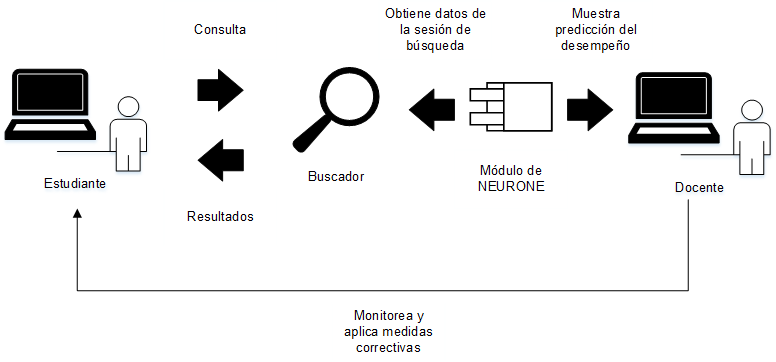
\includegraphics[width=0.9\textwidth]{03_GraphicFiles/monitor.png}
	%\input{03_GraphicFiles/p07.pdf}
	\captionsource{Proceso de búsqueda de información de un estudiante}{\fuentePropia}
	\label{fig:docente_estudiante}
\end{figure}

\section{Alcances y limitaciones de la solución}
\label{sec:alcances}
Los modelos se construyen a partir de un conjunto de datos específicos, estos datos tienen su propio contexto y origen que limitan la generalización de los modelos a construir. A continuación, se describen las principales limitaciones y alcances de la solución.

\begin{enumerate}
	\item El curso de alfabetización informacional y sus respectivos registros de datos, pertenecen al proyecto iFuCo [24], el cual es un trabajo colaborativo entre universidades de Finlandia (University of Tampere, University of Jyväskylä y University of Turku) y de Chile (Universidad de Santiago de Chile y Pontificia Universidad Católica de Chile). 
	\item Los registros de datos provienen de un estudio enmarcado en un curso de alfabetización en información, aplicado al área de Ciencia y Ciencias Sociales, en ambos países.
	\item Los datos son recolectados y almacenados por un sistema externo llamado NEURONE (\ingles{oNlinE inqUiry expeRimentatiON systEm}), trabajo de memoria de un estudiante de la carrera de Ingeniería de Ejecución en Computación e Informática de la Universidad de Santiago de Chile [25].
	\item La solución funciona como un sistema predictor del desempeño de estudiante en la búsqueda de información, sin ofrecer acciones correctivas en caso de bajo desempeño.
\end{enumerate}
\chapter{Metodología, herramientas y ambiente de desarrollo}
\label{ch:metodologia_herramientas_ambiente}

\section{Metodología a usar}
\label{sec:metodologia}
El presente proyecto presenta una componente de investigación y desarrollo de \ingles{software} (I+D). Esto debido a la relación que existe entre ambas componentes, la investigación necesita una herramienta de \ingles{software} de apoyo que permita recibir los datos de NEURONE, alimentar el modelo de predicción y que permita al usuario interactuar con resultados de la predicción a realizar.
\section{Herramientas de desarrollo}
\label{sec:herramientas}
Las herramientas a utilizar en el trabajo de tesis, se dividen tanto en \ingles{hardware} como en \ingles{software}.

\subsection{Herramientas de \ingles{hardware}}
El desarrollo se llevará a cabo con procesador Intel Core i7 7ma Generación \textit{Kabylake} de 3.6 Ghz, con memoria Ram de 16 GB y 2 TB de disco duro. Además, los despliegues de prueba se realizan sobre un servidor privado virtual (VPS, por sus siglas en inglés) con el sistema operativo GNU/Linux Ubuntu Server alojado en el proveedor DigitalOcean\footnote{https://www.digitalocean.com/}.

\subsection{Herramientas de \ingles{software}}
En cuanto herramientas \ingles{software}, el desarrollo se llevará a cabo en la distribución GNU/Linux Debian en su versión 9.0. El modelo se llevará a cabo en Tensorflow. Para el análisis estadístico se hará uso de R. Además, cada módulo desarrollado estará contenido en contenedores de Docker para facilitar el despliegue en producción del modelo desarrollado. Todo el trabajo realizado, tanto código como documento escrito estará bajo el sistema de control de versiones Git. Finalmente, se hará uso de \LaTeX para el documento escrito.
\section{Ambiente}
\label{sec:ambiente}
El ambiente de desarrollo del presente proyecto será tanto en el domicilio particular del candidato a tesista, como también en el Departamento de Ingeniería Informática de la Universidad de Santiago de Chile, específicamente, en el laboratorio de sistemas colaborativos.

Después de finalizar cada iteración, la retroalimentación a este proyecto es ofrecida por miembros del equipo de investigación del proyecto iFuCo y el profesor guía, quien, además brinda apoyo en los aspectos tecnológicos y metodológicos. Finalmente, el equipo de desarrollo de este trabajo de título es unipersonal, con colaboración en fundamentos teóricos de otros tesistas y memoristas involucrados en el proyecto. 


\chapter{Plan de trabajo}
\label{ch:plan_trabajo}

El presente proyecto contempla 612 horas de trabajo efectivas y se realizará en el transcurso del segundo semestre del año 2017, el cual se inicia el 7 de agosto y termina el 7 de diciembre del presente año contemplando 16 semanas de trabajo. Se dispone como día de trabajo todos los días hábiles de la semana, y un horario de trabajo desde las 9:00 hasta las 18:00 hrs considerando una hora de descanso.

El plan de trabajo propuesto se muestra en la \tabla{tab:plan}, dada las metodologías empleadas las actividades se realizan de forma secuencial. Cabe destacar que a la fecha de entrega de este informe, el alumno candidato a tesista ya ha avanzado el estado del arte e investigación de tecnologías.

\begin{table}[htb]
  \centering
    %\captiontable{Plan de trabajo propuesto}{\fuentePropia}
    \captiontable{Plan de trabajo propuesto}
    \pgfplotstabletypeset[
        col sep=semicolon,
        columns/Actividad/.style={string type, column type=|l},
        columns/Duración (HH)/.style={string type},
        display columns/0/.style={column type={p{.7\textwidth}}},
        every even row/.style={before row={\rowcolor[gray]{0.9}}},
        every head row/.style={before row=\toprule,after row=\midrule},
        every last row/.style={after row=\bottomrule}
    ]{04_Tables/plan_trabajo.csv}
    \label{tab:plan}
    \medskip
    \par\centering Fuente: Elaboración propia, (2017)
\end{table}

%\begin{figure}[htb]
%    \centering
%    \scalebox{0.6}{\begin{ganttchart}[
    %today=4
    ]{1}{17}

    \gantttitle{Proyecto tesis}{17}\\
    \gantttitle[]{2017}{17} \\               
    
    \gantttitle{Ago}{4}                     
    \gantttitle{Sep}{4}
    \gantttitle{Oct}{4}
    \gantttitle{Nov}{4}
    \gantttitle{Dic}{1} \\ % Fin: Entrega 7 diciembre 2017
    
    \ganttgroup[inline=false]{Actualización del estado del arte centrado en trabajos recientes}{1}{8} \\ 
    \ganttgroup[inline=false]{Exploración, preprocesamiento y transformación de los registros del proceso de búsqueda de información obtenidos por NEURONE}{1}{17} \\
    \ganttgroup[inline=false]{Definición de las características para la construcción de modelos de predicción del desempeño de búsqueda de estudiantes}{1}{17} \\ 
    \ganttgroup[inline=false]{Comparación y selección de los algoritmos y/o técnicas de minería de datos para la construcción de modelos}{1}{17} \\ 
    \ganttgroup[inline=false]{Validación de los algoritmos y/o técnicas con datos conocidos}{1}{17} \\ 
	\ganttgroup[inline=false]{Evaluación de los modelos construidos utilizando métricas de desempeño}{1}{17} \\ 

    \ganttgroup[progress=70, inline=false]{Redacción del documento}{1}{17} \\ 
\end{ganttchart}}
%    %\begin{ganttchart}[
    %today=4
    ]{1}{17}

    \gantttitle{Proyecto tesis}{17}\\
    \gantttitle[]{2017}{17} \\               
    
    \gantttitle{Ago}{4}                     
    \gantttitle{Sep}{4}
    \gantttitle{Oct}{4}
    \gantttitle{Nov}{4}
    \gantttitle{Dic}{1} \\ % Fin: Entrega 7 diciembre 2017
    
    \ganttgroup[inline=false]{Actualización del estado del arte centrado en trabajos recientes}{1}{8} \\ 
    \ganttgroup[inline=false]{Exploración, preprocesamiento y transformación de los registros del proceso de búsqueda de información obtenidos por NEURONE}{1}{17} \\
    \ganttgroup[inline=false]{Definición de las características para la construcción de modelos de predicción del desempeño de búsqueda de estudiantes}{1}{17} \\ 
    \ganttgroup[inline=false]{Comparación y selección de los algoritmos y/o técnicas de minería de datos para la construcción de modelos}{1}{17} \\ 
    \ganttgroup[inline=false]{Validación de los algoritmos y/o técnicas con datos conocidos}{1}{17} \\ 
	\ganttgroup[inline=false]{Evaluación de los modelos construidos utilizando métricas de desempeño}{1}{17} \\ 

    \ganttgroup[progress=70, inline=false]{Redacción del documento}{1}{17} \\ 
\end{ganttchart}
%    \captionsource{Carta Gantt propuesta.}{\fuentePropia}
%    \label{fig:gantt}
%\end{figure}

\renewcommand{\bibname}{Referencias bibliográficas}
\printbibliography
\addcontentsline{toc}{chapter}{Referencias bibliográficas}
% Start appendix
\appendix

% Appendix A
%%% File encoding is UTF8
%%% You can use special characters just like ä,ü and ñ

\chapter{Capítulo Apéndice}



\section{Sección del apéndice}

\begin{neuralnetwork}[height=4]
\centering
	\newcommand{\nodetextclear}[2]{}
	\newcommand{\nodetextx}[2]{$x_#2$}
	\newcommand{\nodetexty}[2]{$y_#2$}
	\inputlayer[count=4, bias=false, title=Input\\layer, text=\nodetextx]
	\hiddenlayer[count=5, bias=false, title=Hidden\\layer, text=\nodetextclear] \linklayers
	\outputlayer[count=3, title=Output\\layer, text=\nodetexty] \linklayers
\end{neuralnetwork}

\begin{figure}[htb]
	\centering
	\begin{tikzpicture}
	\begin{axis}[axis lines = middle
	, enlargelimits = true
	, xlabel = {$x$}
	, ylabel = {$y$}
	, trig format plots = rad
	, width = 0.9\textwidth
	, height= 80mm
	, cycle list name=Dark2
	, title style={font=\bfseries,align=center,text width=0.7\textwidth}
	, title = {Example Diagram with a Line Break in the Title (using the \texttt{text width} option in the \texttt{title style})},
	]
	\addplot[myColorMainA,domain=0:9, line width=1pt, smooth]
	{0.2*x^2};
	\addplot[myColorMainB,domain=0:9, line width=1pt, smooth]
	{5*sin(x)};
	\end{axis}
	\end{tikzpicture}
	\captionsource{A scientific diagram using the \texttt{pgfplots} package by \textsc{Christian Feuersaenger} using the same colors which are also used for the layout}{\fuentePropia}
	\label{fig:ScientificDiagram}
\end{figure}

\subsection{Subseccion del apéndice}

Como se ve en el \alg{alg:ex1}

\begin{algorithm}[H]
	\caption{\textsc{Escribiendo algoritmos usando \LaTeX2e}}
	\label{alg:ex1}
	\SetAlgoLined
	\KwIn{Esto es la entrada del algoritmo}
	\KwOut{Esto es la salida del algoritmo}
	%\KwData{Esto son los datos con que trabaja el algoritmo}
	%\KwResult{Esto es el resultado del algoritmo}
\Begin{
	$V \longleftarrow U$\;
	$S \longleftarrow \emptyset$\;

	\While{not at end of this document}{
		read current\;
		\eIf{understand}{
			go to next section\;
			current section becomes this one\;
		}{
			go back to the beginning of current section\;
		}
	}
}
\end{algorithm}

% Appendix B
%%% File encoding is UTF8
%%% You can use special characters just like ä,ü and ñ

\chapter{Another Appendix Chapter}


%TODO: fix with cref
%Como se puede apreciar en la \cref{tab:b1}.
Como se puede apreciar en la \tab{tab:b1}.


\insertTableFile{Ejemplo de una tabla}{Elaboración propia, (2017)}{04_Tables/CSVexample.csv}{\label{tab:b1}}



\begin{figure}[!ht]
\centering\makebox[\textwidth]{
\begin{tikzpicture}[node distance =4cm, auto]

    % Place nodes
    \node[block] (susceptible) {Susceptible};
    \node[block, right of=susceptible] (exposed) {Exposed};
    \node[block, right of=exposed] (infectious) {Infectious};
    \node[block, right of=infectious] (removed) {Removed};

\coordinate[below=8mm of susceptible] (bottom brace);

\draw [my brace]
      (exposed.south|-bottom brace) -- (susceptible.south west|-bottom brace) 
      node[bottom label] {
        Environmental \& Human factors
        \begin{itemize}
        \item Foo
        \item Bar
        \item Foobar
        \end{itemize}
      };

\draw [my brace]
    (infectious.south|-bottom brace) -- (exposed.south|-bottom brace)
    node [bottom label] { Variable immunity };

\draw [my brace]
    (removed.south east|-bottom brace) -- (infectious.south|-bottom brace)
    node [bottom label] { 
      Control parameters 
        \begin{itemize}
        \item Foo
        \item Bar
        \end{itemize}
     };    

\coordinate[above=3mm of susceptible] (top brace);

\draw [my brace] 
    (susceptible.north|-top brace) -- (exposed.north|-top brace)
    node [top label] {Contact parameters};

\draw [my brace]
    (exposed.north|-top brace) -- (removed.north|-top brace)
    node[top label] {Disease parameters};

\draw[line] (susceptible) -- (exposed)
            (exposed) -- (infectious)
            (infectious) -- (removed);

\path[line,dashed] 
   (removed.south) -- +(0,-.35) -| (susceptible.south);

\end{tikzpicture}}
\smallskip
\label{fig:flowchart_disease_transmission}
\caption{Flowchart of fundamental disease transmission mechanisms}
\end{figure}

%%%%%%%%%%%%%%%%%%%%%%%%%%%%%%%%%%%%%%%%%%%%%%%%%%%%%%%%%%%%%%%%%%%%%%



%%%%%%%%%%%%%%%%%%%%%%%%%%%%%%%%%%%%%%%%%%%%%%%%%

\begin{tikzpicture}[node distance=5em, scale=2, decoration = brace]
    \def\yTop{0.2};
    \def\yBottom{-0.2};

    % timeline
    \draw [arrow] (0,0) to (3.7,0);
    \draw [] (0,-0.1) to (0,0.1);

    % group 1
    \node [cmdcircle] (c0) at (0.3, 0) {};
    \node[draw=none, fill=none, color = cmdlabel] at (0.3,\yTop) {$c_0$};

    \node [eventcircle] (e0) at (0.6, 0) {};
    \node[draw=none, fill=none, color = eventlabel] at (0.6,\yBottom) {$e_0$};

    \node [eventcircle] (e1) at (0.9, 0) {};
    \node[draw=none, fill=none, color = eventlabel] at (0.9,\yBottom) {$e_1$};

    % group 2
    \node [cmdcircle] (c1) at (1.9, 0) {};
    \node[draw=none, fill=none, color = cmdlabel] at (1.9,\yTop) {$c_1$};

    \node [eventcircle] (e2) at (2.2, 0) {};
    \node[draw=none, fill=none, color = eventlabel] at (2.2,\yBottom) {$e_2$};

    % group 3
    \node [cmdcircle] (c2) at (2.9, 0) {};
    \node[draw=none, fill=none, color = cmdlabel] at (2.9,\yTop) {$c_2$};

    \node [eventcircle] (e3) at (3.2, 0) {};
    \node[draw=none, fill=none, color = eventlabel] at (3.2,\yBottom) {$e_3$};

    \draw [cmdarrow, bend angle=40, bend left] (c0) to (c1);
    \draw [cmdarrow, bend angle=55, bend left] (c1) to (c2);

    \draw [eventarrow, bend angle=55, bend right] (e0) to (e1);
    \draw [eventarrow, bend angle=55, bend right] (e1) to (e2);
    \draw [eventarrow, bend angle=55, bend right] (e2) to (e3);

    % labels
    \node[draw=none,fill=none, color = cmdlabel] at (1.5,0.5) {Replaying Comands};
    \node[draw=none,fill=none, color = eventlabel] at (2,-0.5) {Rebuilding State};

\end{tikzpicture}

%%%%%%%%%%%%%%%%%%%%%%%%%%%%%%%%%%%%%%%%%%%%%%%%%


%%%%%%%%%%%%%%%%%%%%%%%%%%%%%%%%%%%%%%%%%%%%

% Supervised setup

\usetikzlibrary{positioning, decorations.pathmorphing}

\begin{tikzpicture}[node distance=1.5cm]
    \node[rectangle, very thick, draw] (learning) {Learning algorithm, $L$};
    \node[rectangle, very thick, draw, below = of learning] (inference) {Labelling function, $h$};
    \node[left = of learning] (train) {Training data, $\vec{s}$};
    \node[left = of inference] (uns) {Unseen data, $x$};
    \node[right = of inference] (lab) {Label, $y$};
    
    \draw[-stealth, very thick] (train) -- (learning);
    \draw[-stealth, very thick, decoration={snake, segment length=2mm, amplitude=0.3mm, post length=1.5mm}, decorate] (learning) -- node[right] {$L(\vec{s})$} (inference);
    \draw[-stealth, very thick] (uns) -- (inference);
    \draw[-stealth, very thick] (inference) -- node[above] {$h(x)$} (lab);
\end{tikzpicture}

%%%%%%%%%%%%%%%%%%%%%%%%%%%%%%%%%%%%%%%%%%%%

%  CQRS



%%%%%%%%%%%%%%%%%%%%%%%%%%%%%%%%%%%%%%%%%%%%

% SVM

%\begin{tikzpicture}[scale=.8]
%  % Draw axes
%  \draw [<->,thick] (0,5) node (yaxis) [above] {$y$}
%        |- (5,0) node (xaxis) [right] {$x$};
%  % Draw line
%  \draw (0,-1) -- (5,4); % y=x-1
%  \draw[dashed] (-1,0) -- (4,5); % y=x+1
%  \draw[dashed] (2,-1) -- (6,3); % y=x-3
%  % Draw labels
%  \draw (3.5,3) node[rotate=45,font=\small] 
%        {$\mathbf{w}\cdot \mathbf{x} + b = 0$};
%  \draw (2.5,4) node[rotate=45,font=\small] 
%        {$\mathbf{w}\cdot \mathbf{x} + b = 1$};
%  \draw (4.5,2) node[rotate=45,font=\small] 
%        {$\mathbf{w}\cdot \mathbf{x} + b = -1$};
%  % Draw distance
%  \draw[dotted] (4,5) -- (6,3);
%  \draw (5.25,4.25) node[rotate=-45] {$\frac{2}{\Vert \mathbf{w} \Vert}$};
%  \draw[dotted] (0,0) -- (0.5,-0.5);
%  \draw (0,-0.5) node[rotate=-45] {$\frac{b}{\Vert \mathbf{w} \Vert}$};
%  \draw[->] (2,1) -- (1.5,1.5);
%  \draw (1.85,1.35) node[rotate=-45] {$\mathbf{w}$};
%  % Draw negative dots
%  \fill[red]   (1.5,2.5)   circle (3pt);
%  \fill[black] (1,2.5)     circle (3pt);
%  \fill[black] (0.75,2)    circle (3pt);
%  \fill[black] (0.6,1.9)   circle (3pt);
%  \fill[black] (0.77, 2.5) circle (3pt);
%  \fill[black] (1.5,3)     circle (3pt);
%  \fill[black] (1.3,3.3)   circle (3pt);
%  \fill[black] (0.6,3.2)   circle (3pt);
%  % Draw positive dots
%  \draw[red,thick] (4,1)     circle (3pt); 
%  \draw[red,thick] (3.3,.3)  circle (3pt); 
%  \draw[black]     (4.5,1.2) circle (3pt); 
%  \draw[black]     (4.5,.5)  circle (3pt); 
%  \draw[black]     (3.9,.7)  circle (3pt); 
%  \draw[black]     (5,1)     circle (3pt); 
%  \draw[black]     (3.5,.2)  circle (3pt); 
%  \draw[black]     (4,.3)    circle (3pt); 
%\end{tikzpicture}

%%%%%%%%%%%%%%%%%%%%%%%%%%%%%%%%%%%%%%%%%

% Processor

\usetikzlibrary{arrows.meta}
\usetikzlibrary{positioning}
\usetikzlibrary{shapes.geometric}
\usetikzlibrary{calc} 
\tikzstyle{naveqs} = [text width=3.3cm, fill=white, minimum height=3em, rounded corners, text centered, draw=black,
minimum width = 3.3cm
]
\tikzset{
    arrow/.style={-latex, shorten >=0pt, shorten <=0pt},
    arrowboth/.style={<->/.tip = Latex, shorten >=0pt, shorten <=0pt}
}

%-----#1 height, #2 width, #3 aspect, #4 name of the node, #5 coordinate, #6 label
\def\elBox[#1,#2,#3,#4,#5]#6{
    \node[draw, cylinder, alias=cyl, shape border rotate=90, aspect=#3, 
    minimum height=#1, minimum width=#2, outer sep=-0.5\pgflinewidth, 
    fill = white!30,
    %color=orange!40!black, left color=orange!70, right color=orange!80, middle color=white
    ] (#4) at #5 {};

    %\node at #5 [text width=1.5cm, text centered] {#6};
    \node at #5 [text width=1.9cm, text centered] {#6};

    \fill [white!30] let \p1 = ($(cyl.before top)!0.5!(cyl.after top)$), 
        \p2 = (cyl.top), \p3 = (cyl.before top),
        \n1={veclen(\x3-\x1,\y3-\y1)},
        \n2={veclen(\x2-\x1,\y2-\y1)} in (\p1) ellipse (\n1 and \n2); 
}
%-----ABoxes
%-----#1 height, #2 width, #3 aspect, #4 name of the node, #5
%-----coordinate, #6 label
\def\aboxl[#1,#2,#3,#4,#5]#6{%
    \node[draw, cylinder, alias=cyl, shape border rotate=90, aspect=#3, %
    minimum height=#1, minimum width=#2, outer sep=-0.5\pgflinewidth, %
    fill = white!30%
] (#4) at #5 {};%
    \node at #5 [text width=1.5cm, text centered] {#6};%
    \fill [white!30] let \p1 = ($(cyl.before top)!0.5!(cyl.after
    top)$), \p2 =
    (cyl.top), \p3 = (cyl.before top),
    \n1={veclen(\x3-\x1,\y3-\y1)},
    \n2={veclen(\x2-\x1,\y2-\y1)} in (\p1) ellipse (\n1 and
    \n2); }
            

\begin{tikzpicture}
    \def\y{2}
    \def\x{4.0}
    \def\n{0.2}
    \def\shift{5mm}

    \node (cqrs) [roundBox, label={[yshift=-6.8cm]Command Model}, fill = bgcolor0, minimum width = 5cm, minimum height = 6.2cm] at (\x,-1.9cm) {};
    \node (retro) [roundBox, label={[yshift=-6.87cm]Query Model}, fill = bgcolor2, minimum width = 5cm, minimum height = 6.2cm] at (-\x,-1.9cm) {};

    \node (commands) at (\x, 2.1) {Commands};
    \node (queries) at (-\x, 2.1) {Queries};

    \node (commandmodel) [naveqs, fill = white!30] at (\x, 0){Command Processor};
    \draw [arrow] (commands) to (commandmodel);

    \node (ceventlog) [naveqs, fill = white!30] at (\x, -4){Event Log};

    \node (state) [naveqs,  align = center, fill = white!30] at (-\x, 0) {State};
    \node (querymodel) [naveqs,  align = center, fill = white!30] at (-\x, -2) {Event Processor};
    %\draw [arrow] (queries) to (querymodel);
    \node (qeventlog) [naveqs, fill = white!30] at (-\x, -4){Event Log};
    \draw [arrow] 
        (commandmodel) to 
        node[midway, right=0.0em, text centered] {Events}  
        (ceventlog);
    \draw [arrow] 
        (qeventlog) to 
        node[midway, right=0.0em, text centered] {Events}  
        (querymodel);

    \draw [arrow] (querymodel) to (state);

    %\draw [arrow] ([xshift=2cm]querymodel) to ([xshift=2cm]queries);
    % uebler hack
    \draw [arrow] (-\x - \n, 1.8) to (-\x - \n, 0.54);
    \draw [arrow] (-\x + \n, 0.54) to (-\x + \n, 1.8);

    %\draw [arrow] ([transform canvas={xshift=\shift}]querymodel) to ([transform canvas={xshift=\shift}]queries);

    \draw [arrow, dashed] 
        (ceventlog) to 
        node[midway,above=0.0em, text centered] {Publish Events}  
        (qeventlog);

\end{tikzpicture}

%%%%%%%%%%%%%%%%%%%%%%%%%%%%%%%%%%%%%%%%%



\begin{tikzpicture}

\begin{scope}[block/.style={align=center,rectangle,draw=black!100,inner sep=0cm,minimum size=2.3cm,fill=#1!60},
             red block/.style={block=red},
             green block/.style={block=green}]
%Draw the four blocks
\matrix[inner sep=0cm,row sep=0.2cm,column sep=0.2cm,ampersand replacement=\&]{
    \node [block=green] (h)  {\begin{tabular}{c}\textbf{hit}\\\mathcal{H\!i}\end{tabular}};                       \& 
    \node [block=violet]   (fa) {\begin{tabular}{c}\textbf{false alarm}\\\mathcal{F\!A}\end{tabular}} ;    \\
    \node [block=red]   (m)  {\begin{tabular}{c}\textbf{miss}\\\mathcal{M\!i}\end{tabular}} ;                     \&
    \node [block=olive] (cr) {\begin{tabular}{c}\textbf{correct reject}\\\mathcal{C\!R} \end{tabular}} ; \\
};

% Draw the class-labels
\node[above=0.2cm,anchor=base] at (h.north) {Anomaly $(\mathcal{C}_{\text{A}})$};
\node[above=0.2cm,anchor=base] at (fa.north) {Normality $(\mathcal{C}_{\text{N}})$};
\node[left=0.2cm,rotate=90,anchor=base] at (h.west) {Outlier $(\mathcal{C}_{\text{O}})$};
\node[left=0.2cm,rotate=90,anchor=base] at (m.west) {Inlier $(\mathcal{C}_{\text{I}})$};

% Define necessary coordinates
\coordinate (ul) at ($(h.north west)+(0cm,0.6cm)$);
\coordinate (ur) at ($(fa.north east)+(0cm,0.6cm)$);
\coordinate (la) at ($(h.north west)-(0.6cm,0cm)$);
\coordinate (lb) at ($(m.south west)-(0.6cm,0cm)$);

% Draw the two lines
\draw (ul) -- (ur);
\draw (la) -- (lb);

% Draw the ``Expert'' and ``Algorithmic'' labels
\node[above=0.2cm,anchor=base,inner sep=0cm,outer sep=0cm] at ($ (ul)!.5!(ur) $) {Expert labels the observation as a(n)};
\node[left=0.2cm,rotate=90,anchor=base,inner sep=0cm,outer sep=0cm] at ($ (la)!.5!(lb) $) {Algorithm classifies the data point as an};
\end{scope}

%\thesisbb

\end{tikzpicture}

%%%%%%%%%%%%%%%%%%%%%%%%%%%%%%%%%%%%%%%%%%%%%%%%%%%%%%%%%%

% Confusion Matrix

\newcommand\MyBox[2]{
  \fbox{\lower0.75cm
    \vbox to 1.7cm{\vfil
      \hbox to 1.7cm{\hfil\parbox{1.4cm}{#1\\#2}\hfil}
      \vfil}%
  }%
}

\noindent
\renewcommand\arraystretch{1.5}
\setlength\tabcolsep{0pt}
\begin{tabular}{c >{\bfseries}r @{\hspace{0.7em}}c @{\hspace{0.4em}}c @{\hspace{0.7em}}l}
  \multirow{10}{*}{\rotatebox{90}{\parbox{1.1cm}{\bfseries\centering actual\\ value}}} & 
    & \multicolumn{2}{c}{\bfseries Prediction outcome} & \\
  & & \bfseries p & \bfseries n & \bfseries total \\
  & p$'$ & \MyBox{True}{Positive} & \MyBox{False}{Negative} & P$'$ \\[2.4em]
  & n$'$ & \MyBox{False}{Positive} & \MyBox{True}{Negative} & N$'$ \\
  & total & P & N &
\end{tabular}

%%%%%%%%%%%%%%%%%%%%%%%%%%%%%%%%%%%%%%%%%%%%%%%%%%%%%%%%%%

%% Use of forest: https://tex.stackexchange.com/questions/263749/how-to-create-classification-taxonomies-for-literature-review-using-latex


%%%%%%%%%%%%%%%%%%%%%%%%%%%%%%%%%%%%%%%%%%%%%%%%%%%%%%%%%%%


\usetikzlibrary{arrows.meta}
\usetikzlibrary{positioning}
\usetikzlibrary{shapes.geometric}
\usetikzlibrary{calc} 
\tikzstyle{naveqs} = [text width=6em, fill=white, minimum height=5em, rounded corners, text centered, draw=black]
\tikzset{
    arrow/.style={-latex, shorten >=0pt, shorten <=0pt},
    arrowboth/.style={<->/.tip = Latex, shorten >=0pt, shorten <=0pt}
}

%-----#1 height, #2 width, #3 aspect, #4 name of the node, #5 coordinate, #6 label
\def\elBox[#1,#2,#3,#4,#5]#6{
    \node[draw, cylinder, alias=cyl, shape border rotate=90, aspect=#3, 
    minimum height=#1, minimum width=#2, outer sep=-0.5\pgflinewidth, 
    fill = white!30,
    %color=orange!40!black, left color=orange!70, right color=orange!80, middle color=white
    ] (#4) at #5 {};

    %\node at #5 [text width=1.5cm, text centered] {#6};
    \node at #5 [text width=1.9cm, text centered] {#6};

    \fill [white!30] let \p1 = ($(cyl.before top)!0.5!(cyl.after top)$), 
        \p2 = (cyl.top), \p3 = (cyl.before top),
        \n1={veclen(\x3-\x1,\y3-\y1)},
        \n2={veclen(\x2-\x1,\y2-\y1)} in (\p1) ellipse (\n1 and \n2); 
}
%-----ABoxes
%-----#1 height, #2 width, #3 aspect, #4 name of the node, #5
%-----coordinate, #6 label
\def\aboxl[#1,#2,#3,#4,#5]#6{%
  \node[draw, cylinder, alias=cyl, shape border rotate=90, aspect=#3, %
    minimum height=#1, minimum width=#2, outer sep=-0.5\pgflinewidth, %
    fill = white!30%
      ] (#4) at #5 {};%
      \node at #5 [text width=1.5cm, text centered] {#6};%
        \fill [white!30] let \p1 = ($(cyl.before top)!0.5!(cyl.after
        top)$), \p2 =
          (cyl.top), \p3 = (cyl.before top),
          \n1={veclen(\x3-\x1,\y3-\y1)},
        \n2={veclen(\x2-\x1,\y2-\y1)} in (\p1) ellipse (\n1 and
        \n2); }
            

\begin{tikzpicture}

    \node (applogic) [naveqs, minimum width = 10cm, text width = 5cm, fill = blue!10] at (0, 1.3cm) {Application};

    \node (cqrs) [naveqs, label={[anchor=west]}, fill = red!10, minimum width = 10cm, minimum height = 8cm] at (0,-4.0cm) {};

    \node (api) [naveqs] {CQRS Application Interface};

    %\node [tri, shape border rotate=180] (A) {A};

    \node (commandmodel) [naveqs, below right = 10mm and 10mm of api, fill = white!30] {Command Model};
    \draw [arrow, bend angle=25, bend left] 
        (api) to 
        node[midway,right=0.4em] {Commands}  
        (commandmodel);
    %\draw [arrow, bend angle=25, bend left] (commandmodel) to (api);

    \elBox[5.2em,5em,2.0,eventlog, (3.4,-6.5)] { Event\\Log };
    \draw [arrow] 
        ([yshift=0mm]commandmodel) to 
        node[midway,right=0.0em, text centered] {Events}  
        (eventlog);

    \node (querymodel) [naveqs,  below left = 10mm and 10mm of api, align = center, fill = white!30] {Query\\Model};
    \draw [arrow, bend angle=25, bend right] 
        (api) to 
        node[midway,left=0.5em] {Queries}  
        (querymodel);

    \draw [arrow, bend angle=25, bend right] (querymodel) to (api);

    \aboxl[5.2em,5em,2.0,currentstate, (-3.4,-6.5)] { Current State };

    \draw [arrow] 
        (currentstate) to
        node[midway,right=0.0em, text centered, text width = 1.5cm] {Read-only\\Access}  
        ([yshift=-8.7mm]querymodel);

    %\draw [arrow, bend angle=25, bend left, dashed] 
        %(commandmodel) to 
        %node[midway,below=1.4em,text width=2.2cm, text centered] {State Updates (Events)}  
        %(currentstate);

    \draw [arrow, dashed] 
        (eventlog) to 
        node[midway,below=0.3em,text width=2.2cm, text centered] {State Updates (Events)}  
        (currentstate);

    %\path (api) -- (commandmodel) node[draw=none, midway, left]{ Commands };
    %\draw [bend angle=25, bend left] (api) to (commandmodel) {Commands};
    %\draw  (api)  to [bend left=45] node[sloped,midway,above] {midway label} (commandmodel) ;



%\begin{scope}[>=Latex]
%\draw[>->] (0pt,3ex) -- (1cm,3ex);
%\draw[|<-|] (0pt,2ex) -- (1cm,2ex);
%\end{scope}
\end{tikzpicture}




\usetikzlibrary{arrows.meta}
\usetikzlibrary{positioning}
\usetikzlibrary{shapes.geometric}
\usetikzlibrary{calc} 
\tikzstyle{naveqs} = [text width=6em, fill=white, minimum height=5em, rounded corners, text centered, draw=black]
\tikzset{
    arrow/.style={-latex, shorten >=0pt, shorten <=0pt},
    arrowboth/.style={<->/.tip = Latex, shorten >=0pt, shorten <=0pt}
}

%-----#1 height, #2 width, #3 aspect, #4 name of the node, #5 coordinate, #6 label
\def\elBox[#1,#2,#3,#4,#5]#6{
    \node[draw, cylinder, alias=cyl, shape border rotate=90, aspect=#3, 
    minimum height=#1, minimum width=#2, outer sep=-0.5\pgflinewidth, 
    fill = white,
    %color=orange!40!black, left color=orange!70, right color=orange!80, middle color=white
    ] (#4) at #5 {};

    %\node at #5 [text width=1.5cm, text centered] {#6};
    \node at #5 [text width=3.8cm, text centered] {#6};

    \fill [white] let \p1 = ($(cyl.before top)!0.5!(cyl.after top)$), 
        \p2 = (cyl.top), \p3 = (cyl.before top),
        \n1={veclen(\x3-\x1,\y3-\y1)},
        \n2={veclen(\x2-\x1,\y2-\y1)} in (\p1) ellipse (\n1 and \n2); 
}

%-----#1 height, #2 width, #3 aspect, #4 name of the node, #5 coordinate, #6 label
\def\aboxl[#1,#2,#3,#4,#5]#6{
    \node[draw, cylinder, alias=cyl, shape border rotate=90, aspect=#3, 
    minimum height=#1, minimum width=#2, outer sep=-0.5\pgflinewidth, 
    fill = white
    ] (#4) at #5 {};

    \node at #5 [text width=1.5cm, text centered] {#6};

    \fill [white] let \p1 = ($(cyl.before top)!0.5!(cyl.after top)$), 
        \p2 = (cyl.top), \p3 = (cyl.before top),
        \n1={veclen(\x3-\x1,\y3-\y1)}, 
        \n2={veclen(\x2-\x1,\y2-\y1)} in (\p1) ellipse (\n1 and \n2); 
}

\begin{tikzpicture}[decoration=brace]

    \node (applogic) [naveqs, xshift = 52.5mm, minimum width = 20.5cm, text width = 5cm, fill = blue!10] at (-0.05, 1.3cm) {Application};

    \node (cqrs) [naveqs, label={[anchor=west]}, fill = red!10, minimum width = 20.5cm, minimum height = 8cm] at (5.20,-4.0cm) {};

    \node (api) [naveqs] {CQRS Application Interface};

    %\node (where) [align = center, yshift = 15mm, right = 10mm of applogic] {Where are the retroactive\\features available?};

    %\node [tri, shape border rotate=180] (A) {A};

    \node (commandmodel) [naveqs, below right = 10mm and 10mm of api] {Command Model};
    \draw [arrow, bend angle=25, bend left] 
        (api) to 
        node[midway,right=0.4em] {Commands}  
        (commandmodel);

    %\draw [arrow, bend angle=25, bend left] 
        %(commandmodel) 
        %node[midway, yshift=-25mm, xshift=15mm, left=0.0em, align = center] {Event\\Reference}  
        %to (api);

    %\elBox[5.2em,11.5em,2.0,eventlog, (11.7,-6.6)] { Command/Event Log + Retroactive Store };
    \elBox[5.2em,11.5em,2.0,eventlog, (8.3,-6.8)] { Timeline + Retroactive Store };
    \draw [arrow] 
        ([yshift=0mm]commandmodel) to 
        node[midway, left=0.1em, text centered, 
        yshift=0mm, xshift=0mm, 
        text width = 2.5cm] {Commands\\\qquad\quad+ Events}  
        (eventlog);

    \node (querymodel) [naveqs,  below left = 10mm and 10mm of api, align = center] {Query\\Model};
    \draw [arrow, bend angle=25, bend right] 
        (api) to 
        node[midway,left=0.5em] {Queries}  
        (querymodel);

    \draw [arrow, bend angle=25, bend right] (querymodel) to (api);

    \aboxl[5.2em,5em,2.0,currentstate, (-3.4,-6.8)] { Current State };

    %\draw [<->,arrowboth] 
        %([yshift=-3mm]querymodel) to 
        %node[midway,right=0.1em, text centered, align = center] {Read-only\\Access}  
        %(currentstate);

    \draw [arrow] 
        (currentstate) to
        node[midway, right=0.0em, text centered, text width = 1.5cm] {Read-only\\Access}  
        ([yshift=-8.7mm]querymodel);

    %\draw [arrow,  bend left, bend angle = 20, dashed] 
    \draw [arrow,   dashed] 
        ([yshift=0mm]eventlog) to 
        node[midway,below=0.4em,text width=5.9cm, text centered] {State Updates (Events)}  
        ([xshift=9mm]currentstate);

    %\path (api) -- (commandmodel) node[draw=none, midway, left]{ Commands };
    %\draw [bend angle=25, bend left] (api) to (commandmodel) {Commands};
    %\draw  (api)  to [bend left=45] node[sloped,midway,above] {midway label} (commandmodel) ;

    % Retroactive Stuff
    %\node (rapi) [naveqs, yshift = 40mm, right = 44mm of cqrs] {Retroactive Application Interface};

    \node (rcommandmodel) [naveqs, yshift = 0mm, right = 80mm of commandmodel] {Retroactive Operations Model};
    %\draw [arrow, bend angle=8, bend left] 
    \draw [arrow, bend angle = 31, bend left] 
        (commandmodel) to 
        node[midway, above=0.2em, align = center, text width = 4cm] {Retroactive Operations}  
        (rcommandmodel);
    %\draw [arrow, bend angle=8, bend left] 
    \draw [arrow, bend angle= 24, bend right] 
        (rcommandmodel) to 
        %node[midway, below=0.2em, align = center, text width = 4cm] {Event Reference}  
        (commandmodel);

    \node (rquerymodel) [naveqs,  right = 25mm of commandmodel, align = center] {Retroactive Query Model};
    \draw [arrow, bend angle=10, bend left] 
        (commandmodel) to 
        node[midway, below=1.9em, align = center] {Retroactive\\Queries}  
        (rquerymodel);

    \draw [arrow, bend angle=10, bend left] (rquerymodel) to (commandmodel);

    %\draw [arrow, bend angle=10, bend right] 
        %(rcommandmodel) to 
        %node[midway,below=0.7em,text width=2.2cm, text centered] {Events}  
        %(eventlog);

    %\draw [<->,arrowboth] 
    \draw [arrow] 
        (eventlog) to 
        node[midway,right=0.1em, text centered, align = center] {Read-only\\Access}  
        (rquerymodel);

    \draw [arrow] 
        (rcommandmodel) to 
        node[midway,right=0.9em, align = center] {Write\\Access}  
        (eventlog);

    \draw[decorate, yshift=-4ex] (-2.0,-8) -- node[below=0.4ex] {eventually consistent} (-4.5,-8);

    \draw[decorate, yshift=-4ex] (15.0,-8) -- node[below=0.4ex] {always consistent} (2.0,-8);

\end{tikzpicture}


%\begin{figure}[H]
%    \centering
%    \scalebox{0.3}{% tikz defintions
\usepackage{tikz}
\usetikzlibrary{fit}
\usetikzlibrary{arrows.meta}
\usetikzlibrary{positioning}
\usetikzlibrary{shapes.geometric}
\usetikzlibrary{decorations.pathreplacing}
\usetikzlibrary{calc} 
\usetikzlibrary{patterns}

\tikzstyle{roundBox} = [text width=6em, fill=white, minimum height=5em, rounded corners, text centered, draw=black]

\tikzset{
	arrow/.style={-latex, shorten >=0pt, shorten <=0pt},
	arrowboth/.style={<->/.tip = Latex, shorten >=0pt, shorten <=0pt}
}

\usepackage{xcolor}

\definecolor{bgcolor0}{RGB}{255, 231, 231} %red!10
\definecolor{strokecolor0}{RGB}{255, 181, 181} %red!30

\definecolor{bgcolor1}{RGB}{231, 231, 255} %blue!10
\definecolor{bgcolor2}{RGB}{255, 243, 231} %orange!10

\definecolor{unired}{RGB}{165,0,0}
\definecolor{bgcolor3}{RGB}{238, 205, 205} %unired!20

\tikzset{
	cmdarrow/.style={-latex, shorten >=0pt, shorten <=0pt, color = unired},
	eventarrow/.style={-latex, shorten >=0pt, shorten <=0pt, color = blue!60},
	queryarrow/.style={-latex, shorten >=0pt, shorten <=0pt, color = blue!60},
	cmdcircle/.style={circle, draw, minimum size=5, inner sep=0pt, fill=unired},
	querycircle/.style={circle, draw, minimum size=5, inner sep=0pt, fill=blue!60},
	eventcircle/.style={circle, draw, minimum size=5, inner sep=0pt, fill=blue!60}
}

\definecolor{cmdlabel}{RGB}{165, 0, 0} 
\definecolor{eventlabel}{RGB}{102, 102, 255}
\definecolor{querylabel}{RGB}{102, 102, 255} 

%\begin{document}

%-----#1 height, #2 width, #3 aspect, #4 name of the node, #5 coordinate, #6 label
\def\repositoryA[#1,#2,#3,#4,#5]#6{
	\node[
		draw, cylinder, alias=cyl, shape border rotate=90, aspect=#3, 
		minimum height=#1, minimum width=#2, outer sep=-0.5\pgflinewidth, 
		fill = white,
	] (#4) at #5 {};

	\node at #5 [text width=1.9cm, text centered] {#6};

	\fill [white] let \p1 = ($(cyl.before top)!0.5!(cyl.after top)$), 
		\p2 = (cyl.top), \p3 = (cyl.before top),
		\n1={veclen(\x3-\x1,\y3-\y1)},
		\n2={veclen(\x2-\x1,\y2-\y1)} in (\p1) ellipse (\n1 and \n2); 
}

% defines a box for the repositories (the storages)
%-----#1 height, #2 width, #3 aspect, #4 name of the node, #5 coordinate, #6 label
\def\repositoryB[#1,#2,#3,#4,#5]#6{
	\node[
		draw, cylinder, alias=cyl, shape border rotate=90, aspect=#3, 
		minimum height=#1, minimum width=#2, outer sep=-0.5\pgflinewidth, 
		fill = white
	] (#4) at #5 {};

	\node at #5 [text width=1.5cm, text centered] {#6};

	\fill [white] let \p1 = ($(cyl.before top)!0.5!(cyl.after top)$), 
		\p2 = (cyl.top), \p3 = (cyl.before top),
		\n1={veclen(\x3-\x1,\y3-\y1)},
		\n2={veclen(\x2-\x1,\y2-\y1)} in (\p1) ellipse (\n1 and \n2); 
}
		    

\begin{tikzpicture}[decoration=brace]

	\node (applogic) [roundBox, xshift = 52.5mm, minimum width = 20.5cm, text width = 5cm, fill = bgcolor1] at (0, 1.3cm) {Application};

	\node (cqrs) [roundBox, label={[anchor=west]}, fill = bgcolor0, minimum width = 10cm, minimum height = 8cm] at (0,-4.0cm) {};
	\node (retro) [roundBox, label={[anchor=west]}, fill = bgcolor2, minimum width = 10cm, minimum height = 8cm] at (10.5,-4.0cm) {};

	\node (api) [roundBox] {CQRS Application Interface};


	%\node (where) [align = center, yshift = 15mm, right = 10mm of applogic] {Where are the retroactive\\features available?};

	%\node [tri, shape border rotate=180] (A) {A};

	\node (commandmodel) [roundBox, below right = 10mm and 10mm of api] {Command Model};
	\draw [arrow, bend angle=25, bend left] 
		(api) to 
		node[midway,right=0.4em] {Commands}  
		(commandmodel);
	%\draw [arrow, bend angle=25, bend left, loosely dotted] 
		%(commandmodel) to 
		%node[midway,left=-3mm,yshift=-4mm,align=center] {Event\\Reference}  
		%(api);

	\repositoryA[5.2em,5em,2.0,eventlog, (3.4,-6.5)] { Event\\Log };
	\draw [arrow] 
		([yshift=0mm]commandmodel) to 
		node[midway,right=0.0em, text centered] {Events}  
		(eventlog);

	\node (querymodel) [roundBox,  below left = 10mm and 10mm of api, align = center] {Query\\Model};
	\draw [arrow, bend angle=25, bend right] 
		(api) to 
		node[midway,left=0.5em] {Queries}  
		(querymodel);

	\draw [arrow, bend angle=25, bend right] (querymodel) to (api);

	\repositoryB[5.2em,5em,2.0,currentstate, (-3.4,-6.5)] { Current State };

	%\draw [<->,arrowboth] 
		%([yshift=-3mm]querymodel) to 
		%node[midway,right=0.1em, text centered, align = center] {Read-only\\Access}  
		%(currentstate);

	\draw [arrow] 
		(currentstate) to
		node[midway,right=0.0em, text centered, text width = 1.5cm] {Read-only\\Access}  
		([yshift=-8.7mm]querymodel);

	%\draw [arrow, bend angle=25, bend left, dashed] 
		%(commandmodel) to 
		%node[midway,below=1.4em,text width=2.2cm, text centered] {State Updates (Events)}  
		%(currentstate);

	\draw [arrow, dashed] 
		(eventlog) to 
		node[midway,below=0.3em,text width=2.2cm, text centered] {State Updates (Events)}  
		(currentstate);


	% Retroactive Stuff
	\node (rapi) [roundBox, yshift = 40mm, right = 44mm of cqrs] {Retroactive Application Interface};

	\node (rcommandmodel) [roundBox, below right = 10mm and 10mm of rapi] {
		%\footnotesize
		Retroactive Operations Model
	};
	\draw [arrow, bend angle=25, bend left] 
		(rapi) to 
		node[midway, right=0.8em, align = center] {Retroactive\\Operations}  
		(rcommandmodel);
	\draw [arrow, bend angle=25, bend left] (rcommandmodel) to (rapi);

	\node (rquerymodel) [roundBox,  below left = 10mm and 10mm of rapi, align = center] {
		%\footnotesize
		Retroactive Query Model
	};
	%Retroactive Query Model + Application Query Model};
	\draw [arrow, bend angle=25, bend right] 
		(rapi) to 
		node[midway, left=0.4em, align = center] {Retroactive\\Queries}  
		(rquerymodel);

	\draw [arrow, bend angle=25, bend right] (rquerymodel) to (rapi);
	\repositoryA[5.2em,6em,2.0,rstore, (10.6,-6.5)] { Retroactive\\Store };

	\draw [<->,arrow] 
		%([yshift=-3mm]rquerymodel) to 
		(rstore) to 
		node[midway,left=0.7em, text centered, align = center] {Read-only\\Access}  
		(rquerymodel);

	\draw [<->,arrow] 
		([yshift=-3mm]rcommandmodel) to 
		node[midway,right=0.7em, align = center] {Write\\Access}  
		(rstore);

	\draw[decorate, yshift=-4ex] (5,-8) -- node[below=0.4ex] {eventually consistent} (-5,-8);

	\draw[decorate, yshift=-4ex] (15.5,-8) -- node[below=0.4ex] {always consistent} (5.5,-8);

	\draw [arrow,dotted] 
		(eventlog) to 
		node[midway,below=0.1em, text centered, align = center] {Read-only\\Access}  
		(rstore);

\end{tikzpicture}}
%    \captionsource{Architecture}{\fuentePropia}
%    \label{fig:architecture-example}
%\end{figure}

\end{document}
% ------------------------------------------------------------------
%
% #######################
% End: Document
% #######################
